\section{Background Estimation and Subtraction}
\label{sec:BackgroundSubtraction}

The selected sample contains signal events as well as events coming from various backgrounds. To compute the cross section, we need to subtract background and estimate how many events in each $P_T^\gamma$ bin originate from the $W\gamma$ process. Main sources of backgrounds include jets misidentified as photons denoted as the jets$\rightarrow\gamma$ background, electrons misidentified as photons denoted as the $e\rightarrow\gamma$ background, and backgrounds with real photons denoted as the real-$\gamma$ background. Jets$\rightarrow\gamma$ and real-$\gamma$ backgrounds are present in both channels while $e\rightarrow\gamma$ background is only present in the electron channel. The reminder of this chapter describes the procedure of the background estimation and provides the results.

\subsection{Background from Jets Faking Photons}
\label{sec:BackgroundSubtraction_jtog}

The selected sample is dominated by the $W$+jets background which cannot be further significantly reduced without reducing our signal sample $W\gamma$ as well. The photon~ID selection criteria help to reduce $W$+jets background to a certain level but there is still a significant number of jets that are reconstructed as photons and pass all the photon~ID criteria. DY+jets is another source of the jets$\rightarrow \gamma$ background but this source is significantly suppressed by the $M_W^T$ selection criterion in both channels and by the $Z$-mass window requirement in the electron channel.

The template method is used to estimate jets$ \rightarrow \gamma$ background. First of all, we choose a variable that has a significant discriminative power between the true and fake photon candidates $V_{fit}$. After that, we prepare real-$\gamma$ ($T_{true}$) and fake-$\gamma$ ($T_{fake}$) templates which should be accurate representations of $V_{fit}$ distributions of real and fake photons in the $W\gamma$-selected dataset. The $V_{fit}$ distribution in data is fitted by the following function: 
\begin{equation}\label{eq:F_fit}
F(V_{fit})=N_{true} \cdot T_{true}(V_{fit}) + N_{fake} \cdot T_{fake}(V_{fit}),
\end{equation}
\noindent{where $V_{fit}$ is a fit variable, $N_{true}$ and $N_{fake}$ are numbers of real and fake photons in the data sample, respectively, and $F(V_{fit})$ is a fit function. $N_{true}$ and $N_{fake}$ are fit parameters. We use the charged hadron isolation $I_{ch}^{\gamma}$ and a variable representing ECal shower shape width, $\sigma_{i\eta i\eta}^{\gamma}$, as $V_{fit}$. Results of $I_{ch}^{\gamma}$ fits are further propagated for the cross section calculation, and results of $\sigma_{i\eta i\eta}^{\gamma}$ fits are used for the estimation of the systematic uncertainty.}

% EXPLAIN WHAT IS I_{CH}^{\gamma} and WHAT IS SIHIH
The $I_{ch}^{\gamma}$ is defined as
\begin{equation}
  I_{ch}^{\gamma} = \sum_{ch} P_T,
\end{equation} 
\noindent{where the sum runs over charged hadrons candidates reconstructed by the particle flow algorithm within $\Delta R<0.3$ from the photon.}

The $\sigma_{i\eta i\eta}^{\gamma}$ is defined as
\begin{equation}
  \sigma_{i\eta i\eta}^{\gamma} = \frac{\sum{(\eta_i-\eta)^2 w_i}}{\sum(w_i)},
\end{equation}
\noindent{where the sum runs over~$5\times5$ matrix of crystals around the crystal with the largest $P_T$, and $w_i$ is the weight that has a logarithmic dependence on energy released by the photon.}

To prepare templates, we use $Z\gamma$-selected dataset. $Z\gamma$ goes through two different mechanisms: FSR, when a photon is radiated from one of the final state leptons, and ISR, when a photon is radiated from the initial state quark or antiquark. Real-$\gamma$ templates $T_{true}$ are taken from the FSR events of $Z\gamma\rightarrow\mu\mu\gamma$ while fake-$\gamma$ templates are taken from the ISR events of $Z\gamma\rightarrow\mu\mu\gamma$.

The FSR $Z\gamma$ selection has muon-photon separation requirement of $\Delta R_{min}(\mu,\gamma)>0.4$. This requirement is chosen to be smaller than nominal separation requirement of $\Delta R_{min}(\mu,\gamma)>0.7$ because FSR events typically have smaller separation than ISR events and, therefore, smaller separation increases a fraction of FSR events. Three-particle invariant mass required to be $M_{\gamma\mu\mu}<101$~GeV. 

The FSR contribution drops fast as a function of $P_{T}^{\gamma}$, therefore, the FSR sample has a small statistical power in high $P_{T}^{\gamma}$ bins. To increase the statistical power, we use events from several $P_T^{\gamma}$ ranges to prepare templates for each of them. The distribution of $I_{ch}^{\gamma}$ of real photons does not depend on $P_{T}^{\gamma}$ and, therefore, all events with $P_{T}^{\gamma}>15$~GeV are used to prepare $I_{ch}^{\gamma}$ templates for all $P_T^{\gamma}$ bins. Distributions of $\sigma_{i\eta i\eta}^{\gamma}$ depend on $P_T^{\gamma}$. Only events of $P_T^{\gamma}>30$~GeV are combined together to prepare templates for all $P_T^{\gamma}>30$~GeV bins. Both $I_{ch}^{\gamma}$ and $\sigma_{i\eta i\eta}^{\gamma}$ templates are prepared separately for barrel and endcap photons.

To prepare fake-$\gamma$ templates, we need a sample that consists of jets reconstructed and identified as photons. To prepare such sample, we apply ISR $Z\gamma$ selection conditions on double muon dataset. These selection conditions include nominal $Z\gamma$ selection described in Ch.~\ref{sec:AN_Selection_EventLevel} with tighter requirement on the lepton-photon separation $\Delta{R_{min}}(\mu,\gamma)>1.0$, and a requirement on the invariant mass of the three final state particles $M_{ll\gamma}>101$~GeV. A sample prepared in such a way consists of $Z\gamma$+(DY+jets) events, and jets from the DY+jets are reconstructed and identified as photons same as jets from $W$+jets, DY+jets and $t\bar{t}$+jets in a $W\gamma$-selected sample. 

Therefore, to construct a fake-$\gamma$ template, we can use DY+jets events from the ISR $Z\gamma$-selected sample. However, in addition to DY+jets events, this sample also contains non-negligible amount of $Z\gamma$ events. This real-$\gamma$ contribution is subtracted using $Z\gamma$ MC predictions.

FSR and ISR selections are illustrated in App.~\ref{sec:ZgFSRandISRplots}. Distributions of $M_{ll\gamma}$ and $M_{ll}$ for nominally selected $Z\gamma$ dataset are shown in Fig.~\ref{fig:Zg_Mleplep_and_Mpholeplep}. Distributions of $\Delta{R}(l,\gamma)$ for ISR and FSR $Z\gamma$ events are shown in Fig.~\ref{fig:Zg_ISRandFSR_dR}. Distributions of $P_{T}^{\gamma}$ for ISR and FSR $Z\gamma$ events are shown in Fig.~\ref{fig:Zg_ISRandFSR_phoEt}. 

Fits are performed in the extended binned maximum likelihood manner separately in each $P_T^{\gamma}$ bin, separately for EB and EE photons. Plots of the template fits are available in App.~\ref{sec:TemplateFitPlots}. The outcomes of the fits are parameters $N_{true}$ and $N_{fake}$ from Eq.~\ref{eq:F_fit}.

$N_{true}$ appears to be a number of real-$\gamma$ events in $W\gamma$ dataset after all selection criteria applied except the selection condition on $V_{fit}$ which is either $I_{ch}^{\gamma}$ or $\sigma_{i\eta i\eta}^{\gamma}$. However, our goal is to extract number of real-$\gamma$ events in $W\gamma$ dataset after all selection criteria applied including the selection condition on $V_{fit}$. To extract real-$\gamma$ yield, $N_{true}$ is multiplied by the efficiency of the selection condition on $V_{fit}$. The efficiency is estimated using the $Z\gamma$-selected FSR sample as 
\begin{equation}
 \epsilon_{Vfit} = \frac{N_{passed\_Vfit\_condition}}{N_{failed\_Vfit\_condition}+N_{passed\_Vfit\_condition}},
\end{equation}
\noindent{where $N_{passed\_Vfit\_condition}$ is a number of events in a specific $P_T^{\gamma}$ range is the FSR sample which pass all $Z\gamma$ FSR selection criteria including the selection condition on $V_{fit}$, and $N_{failed\_Vfit\_condition}$ is a number of events in a specific $P_T^{\gamma}$ range in the FSR sample which pass all $Z\gamma$ FSR selection criteria except the selection condition on $V_{fit}$.}

%To extract fake-$\gamma$ yield from the $N_{fake}$, efficiency of the $V_{fit}$ is applied on the value derived from fit based on the distribution of events which are used to prepare a fake-$\gamma$ template. 

\subsection{Background from Electrons Faking Photons in the Electron Channel}
\label{sec:BackgroundSubtraction_etog}

For the electron channel, DY+jets is the main source of the $e \rightarrow \gamma$ background. The $Z$-mass window requirement of ($M_{e\gamma}<70$~GeV or $M_{e\gamma}>110$~GeV) significantly suppresses this background, however, the remaining contribution is non-negligible. 

The contribution of $e\rightarrow\gamma$ $N_{data-nom}^{e\rightarrow\gamma}$ is estimated separately for each $P_{T}^{\gamma}$ bin and separately for barrel and endcap photons by scaling number of the nominally selected events in DY+jets MC sample $N_{MC-nom}^{e\rightarrow\gamma}$ to the relation of numbers of events in the  $e\rightarrow\gamma$-enriched data ($N_{data-Zpeak}^{e\rightarrow\gamma}$) and DY+jets MC ($N_{MC-Zpeak}^{e\rightarrow\gamma}$) samples under the $Z$-peak: 

\begin{equation}\label{eq:Scale_etog}
N_{data-nom}^{e\rightarrow\gamma} = N_{MC-nom}^{e\rightarrow\gamma} \cdot \frac{N_{data-Zpeak}^{e\rightarrow\gamma}}{N_{MC-Zpeak}^{e\rightarrow\gamma}}. 
\end{equation}

To estimate $N_{data-Zpeak}^{e\rightarrow\gamma}$, $e\rightarrow\gamma$-enriched data and DY+jets MC samples are prepared by applying all $W\gamma$ selection requirements except the $Z$-mass window requirement. After that, numbers of events in DY+jets MC samples $N_{MC-Zpeak}^{e\rightarrow\gamma}$ and $N_{MC-nom}^{e\rightarrow\gamma}$ are estimated by counting. The number $N_{data-Zpeak}^{e\rightarrow\gamma}$ is extracted from fitting the $M_{e\gamma}$ distribution in the $Z$-peak region.

The fits are performed in an extended unbinned maximum likelihood manner, separately in each $P_T^\gamma$ bin in fine $\eta^\gamma$ binning. The $\eta^\gamma$ binning for different $P_T^\gamma$ ranges is described in Tab.~\ref{tab:fine_eta_binning}:

\begin{table}[h]
  \small
  \begin{center}
    \caption{Fine $\eta^{\gamma}$ binning for fits for $e\rightarrow\gamma$ background estimation.}
    \begin{tabular}{|c|c|c|}
      \hline
      $P_T^{\gamma}$ ranges, GeV & $\eta^{\gamma}$ binning in barrel &$\eta^{\gamma}$ binning in endcap  \\ \hline
      15-20-25-30-35-45-55-65 & 0.00-0.10-0.50-1.00-1.44 & 1.56-2.10-2.20-2.40-2.50  \\ \hline
      65-75-85-95 & 0.00-0.50-1.44 & 1.56-2.20-2.50  \\ \hline
      95-120-500 & 0.00-1.44 & 1.56-2.50  \\ \hline
      10-15 (underflow) & \multicolumn{2}{|c|}{no fits; MC prediction used} \\ \hline
    \end{tabular}
    \label{tab:fine_eta_binning}
  \end{center}
\end{table} 


The fit model is composed by the template-based function $RooNDKeysPdf$~\cite{ref_RooFit} convoluted with the Gaussian distribution multiplied by the number of events from the $e\rightarrow\gamma$ background  $N_{e\rightarrow\gamma}$ and the function describing a cumulative contribution of all other processes $RooCMSShapePdf$~\cite{ref_RooCMSShapePdf} multiplied by the number of events from other sources that have $M_{e\gamma}$ distributions without a peak at the values of $Z$ mass $N_{else}$. The expression for the fit function is:
\begin{equation}\label{eq:fit_function_etog}
F_{fit}^{e\rightarrow\gamma} = N_{e\rightarrow\gamma} \cdot (RooNDKeysPdf \ast Gaussian) +  N_{else} \cdot (RooCMSShapePdf).
\end{equation}

The function $RooNDKeysPdf$ is a function of the RooFit package~\cite{ref_RooFit} that creates a continuous probability distribution function out of a template. The templates are prepared from $e\rightarrow\gamma$-enriched DY+jets MC sample, separately for each $P_T^{\gamma}$ and $\eta^\gamma$ range. $RooNDKeysPdf$ is convoluted with the Gaussian distribution, the two parameters of the Gaussian distribution are fit parameters. 

The function $RooCMSShapePdf$~\cite{ref_RooCMSShapePdf} is a product of an exponential decay and a constant that smoothly turns over due to a threshold effect. $RooCMSShapePdf$ is described by four parameters, and they all are used as fit parameters in $F_{fit}^{e\rightarrow\gamma}$. Overall,  $F_{fit}^{e\rightarrow\gamma}$ has eight fit parameters, including two parameters of the Gaussian distribution, four parameters of $RooCMSShapePdf$, $N_{e\rightarrow\gamma}$ and $N_{else}$.

The fit plots are provided in App.~\ref{sec:EtogammaFitPlots} and the tables with numbers from Eq.~\ref{eq:Scale_etog} in different $P_T^{\gamma}$ ranges separately for EB and EE final state photons are provided in App.~\ref{sec:etogTables}. The distributions of $M_{e\gamma}$ in different $P_T^{\gamma}$ bins are shown in App.~\ref{sec:Mpholep1DatavsMC}. After the $M_{e\gamma}$ distribution in the DY+jets sample is scaled by 
\begin{equation}
   scale = \frac{N_{data-Zpeak}^{e\rightarrow\gamma}}{N_{MC-Zpeak}^{e\rightarrow\gamma}},
\end{equation}
 \noindent{the data vs MC agreement significantly improves.}

%  \item templates for RooNDKeysPdf: $e\rightarrow\gamma$ portion of the DYjets MC separately for each pt-eta bin
%  \item $e\rightarrow\gamma$ portion of the DYjets MC: a photon has a gen-level electron within dR=0.4 


\subsection{Other Backgrounds}

In addition to the backgrounds discussed before, there is also real-$\gamma$ background. The contributions to this background from $Z\gamma$ and $W\gamma \rightarrow \tau \nu \gamma$ are estimated based on MC predictions.

\begin{itemize}
   \item real-$\gamma$ background from $WW\gamma$;  
   \item $e \rightarrow \gamma$ background in the muon channel. Sources of these backgrounds are $WW$ ($W \rightarrow \mu\nu_{\mu}$ + $W \rightarrow e\nu_e$), $WZ$ ($W \rightarrow \mu\nu_{\mu}$ + $Z \rightarrow ee$ or $W \rightarrow e\nu_{\mu}$ + $Z \rightarrow \mu\mu$) and $ZZ$ ($Z \rightarrow \mu\mu$ + $Z \rightarrow ee$);
   \item fake lepton + real-$\gamma$ ($\gamma$+jets and $\gamma\gamma$+jets events); 
   \item fake lepton + fake-$\gamma$ (multijets events).  
\end{itemize}

\subsection{$P_T^{\gamma}$ Spectra before and after the Background Subtraction}

The results of the background estimation and subtraction procedure are summarized in Fig.~\ref{fig:DDvsMC_Wg_Data_MUON}-\ref{fig:DDvsMC_Wg_Data_ELECTRON} and in Tab.~\ref{tab:yields_Wg_to_munu_}-\ref{tab:yields_Wg_to_enu_}. Figure~\ref{fig:DDvsMC_Wg_Data_MUON} and Tab.~\ref{tab:yields_Wg_to_munu_} stand for the muon channel while Fig.~\ref{fig:DDvsMC_Wg_Data_ELECTRON} and Tab.~\ref{tab:yields_Wg_to_enu_} stand for the electron channel. Top and middle plots in Fig.~\ref{fig:DDvsMC_Wg_Data_MUON}-\ref{fig:DDvsMC_Wg_Data_ELECTRON} shows the $P_T^\gamma$ spectrum in data superimposed with the signal MC and background estimates that includes jets$\rightarrow\gamma$ and real-$\gamma$ backgrounds in both channels and $e\rightarrow\gamma$ background in the electron channel. The bottom plots show data yields after full background subtraction superimposed with signal MC. 

Jets$\rightarrow\gamma$ background is estimated by two methods: by fits of $I_{ch}^{\gamma}$ and $\sigma_{i\eta i\eta}^{\gamma}$ templates. The results provided by two methods differ significantly, as well as both show significant disagreement with the MC prediction. To understand the disagreements and validate the procedure, we perform two MC closure checks. The results of the checks are reported in App.~\ref{sec:MCclosureCheck}.  

For the first MC closure check, the pseudodata sample is prepared from $W$+jets and $W\gamma$ samples and mixed together to mimic real data. Templates are prepared from exactly the same $W\gamma$ and $W$+jets samples that constitute pseudodata. Then fits on this sample of pseudodata are performed and real-$\gamma$ and fake-$\gamma$ fit results are compared to $W\gamma$ and $W$+jets MC predictions. Such approach eliminates effects of possible wrong normalizations of MC samples and the difference between real-$\gamma$ and fake-$\gamma$ $I_{ch}^{\gamma}$ and $\sigma_{i\eta i\eta}^{\gamma}$ distributions in $W\gamma$/W+jets and $Z\gamma$/DY+jets samples. The agreement is quite good between real-$\gamma$ yields extracted from fits and the $W\gamma$ MC prediction. However, the fake-$\gamma$ yields extracted from fits do not always agree that well with $W$+jets MC predictions.

The second check is more realistic: MC samples $W\gamma$, $W$+jets, $Z\gamma$, $Z$+jets, and $t\bar{t}$+jets run through the $W\gamma$ selection conditions and mixed together. To prepare templates, $Z\gamma$ and $DY$+jets MC samples are mixed together to constitute a $Z\gamma$-selected pseudodataset which is used the same way as $Z\gamma$-selected dataset is used to prepare templates for the background estimation in the data analisys. Then the pseudodata histograms are fitted and the fit results are superimposed with MC predictions same as it is done for the real data. Such closure check eliminates the effects of possible wrong normalizations of MC samples but leaves the effect of the possible difference between real-$\gamma$ and fake-$\gamma$ $I_{ch}^{\gamma}$ and $\sigma_{i\eta i\eta}^{\gamma}$ distributions in $W\gamma$/W+jets and $Z\gamma$/DY+jets samples. The results of this closure check show better agreement of data vs estimated background + signal MC however the disagreement in certain $P_T^{\gamma}$ bins remain significant. Presumably, there is a systematic bias in our fit procedure, and it is taken into account as a difference between fit outcomes of the $I_{ch}^{\gamma}$ and $\sigma_{i\eta i\eta}^{\gamma}$ templates as described in detail in Ch.~\ref{sec:Systematics}.

In addition to the checks described above, we also perform $Z\gamma$ check on data and MC mixture (App.~\ref{sec:ZgCheck}). Both $Z\gamma$ data analysis and $Z\gamma$ MC closure check show very good agreement between data and background estimates + signal MC as well as between two methods of the background estimation.

\begin{figure}[htb]
  \begin{center}
   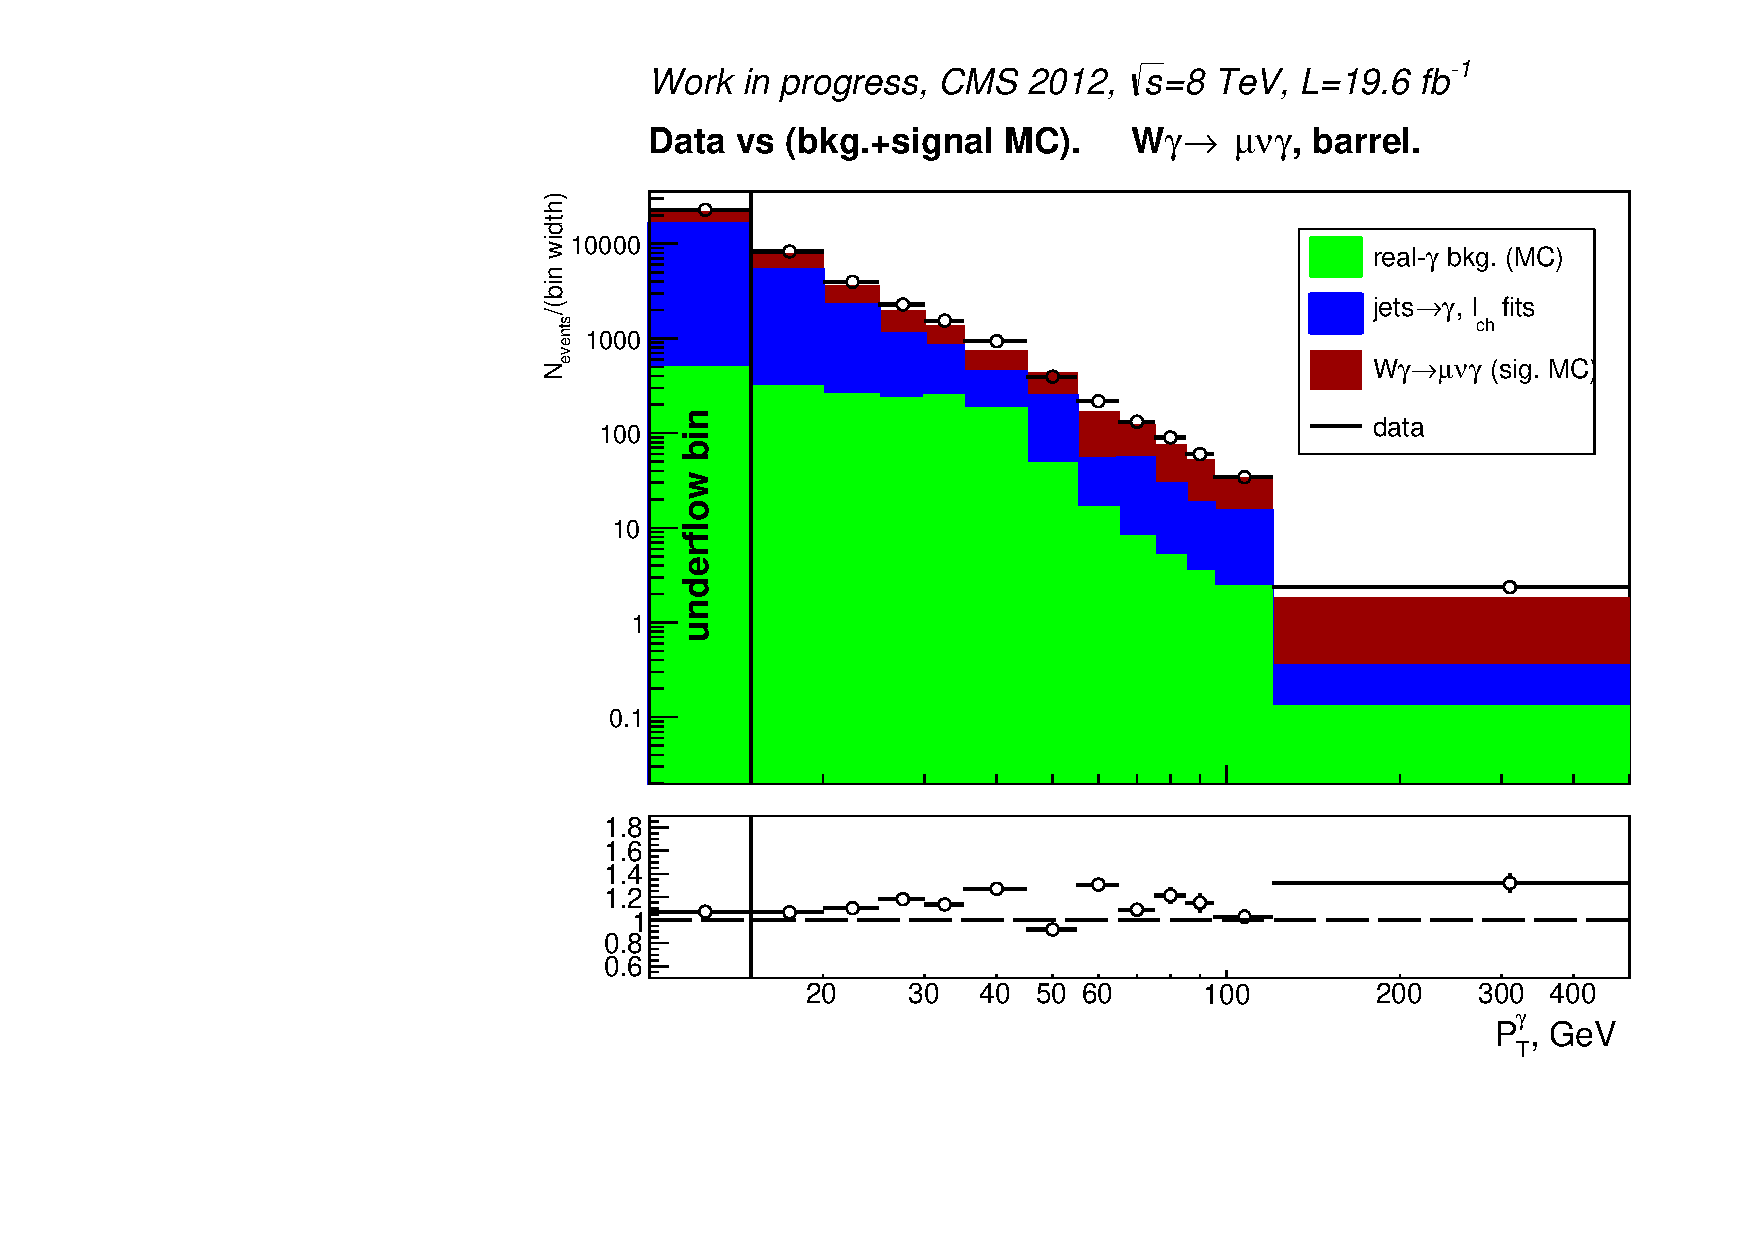
\includegraphics[width=0.45\textwidth]{../figs/figs_v11/MUON_WGamma/PrepareYields/c_DATAvsBkgPlusSigMCc_MUON_WGamma_TEMPL_CHISO_UNblind__Barrel__phoEt.pdf}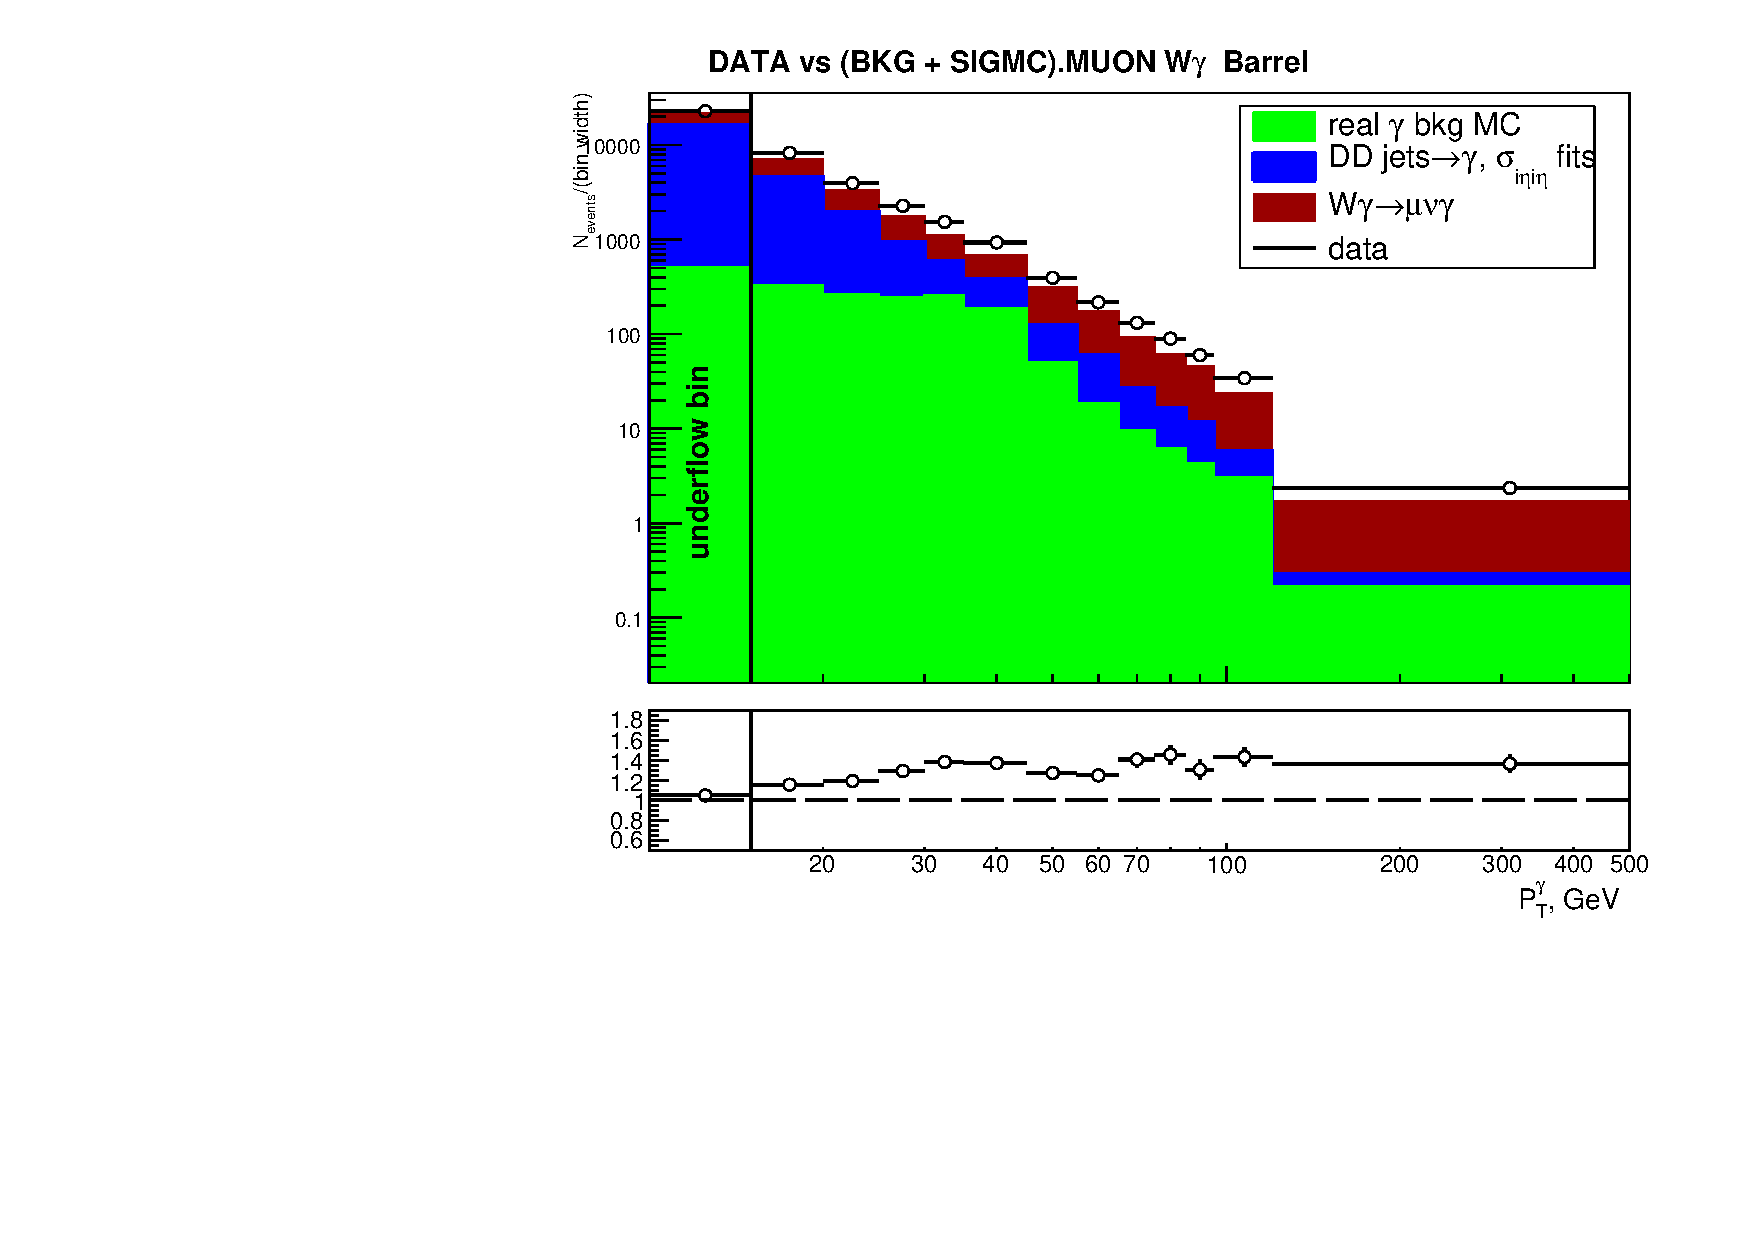
\includegraphics[width=0.45\textwidth]{../figs/figs_v11/MUON_WGamma/PrepareYields/c_DATAvsBkgPlusSigMCc_MUON_WGamma_TEMPL_SIHIH_UNblind__Barrel__phoEt.pdf}  \\
   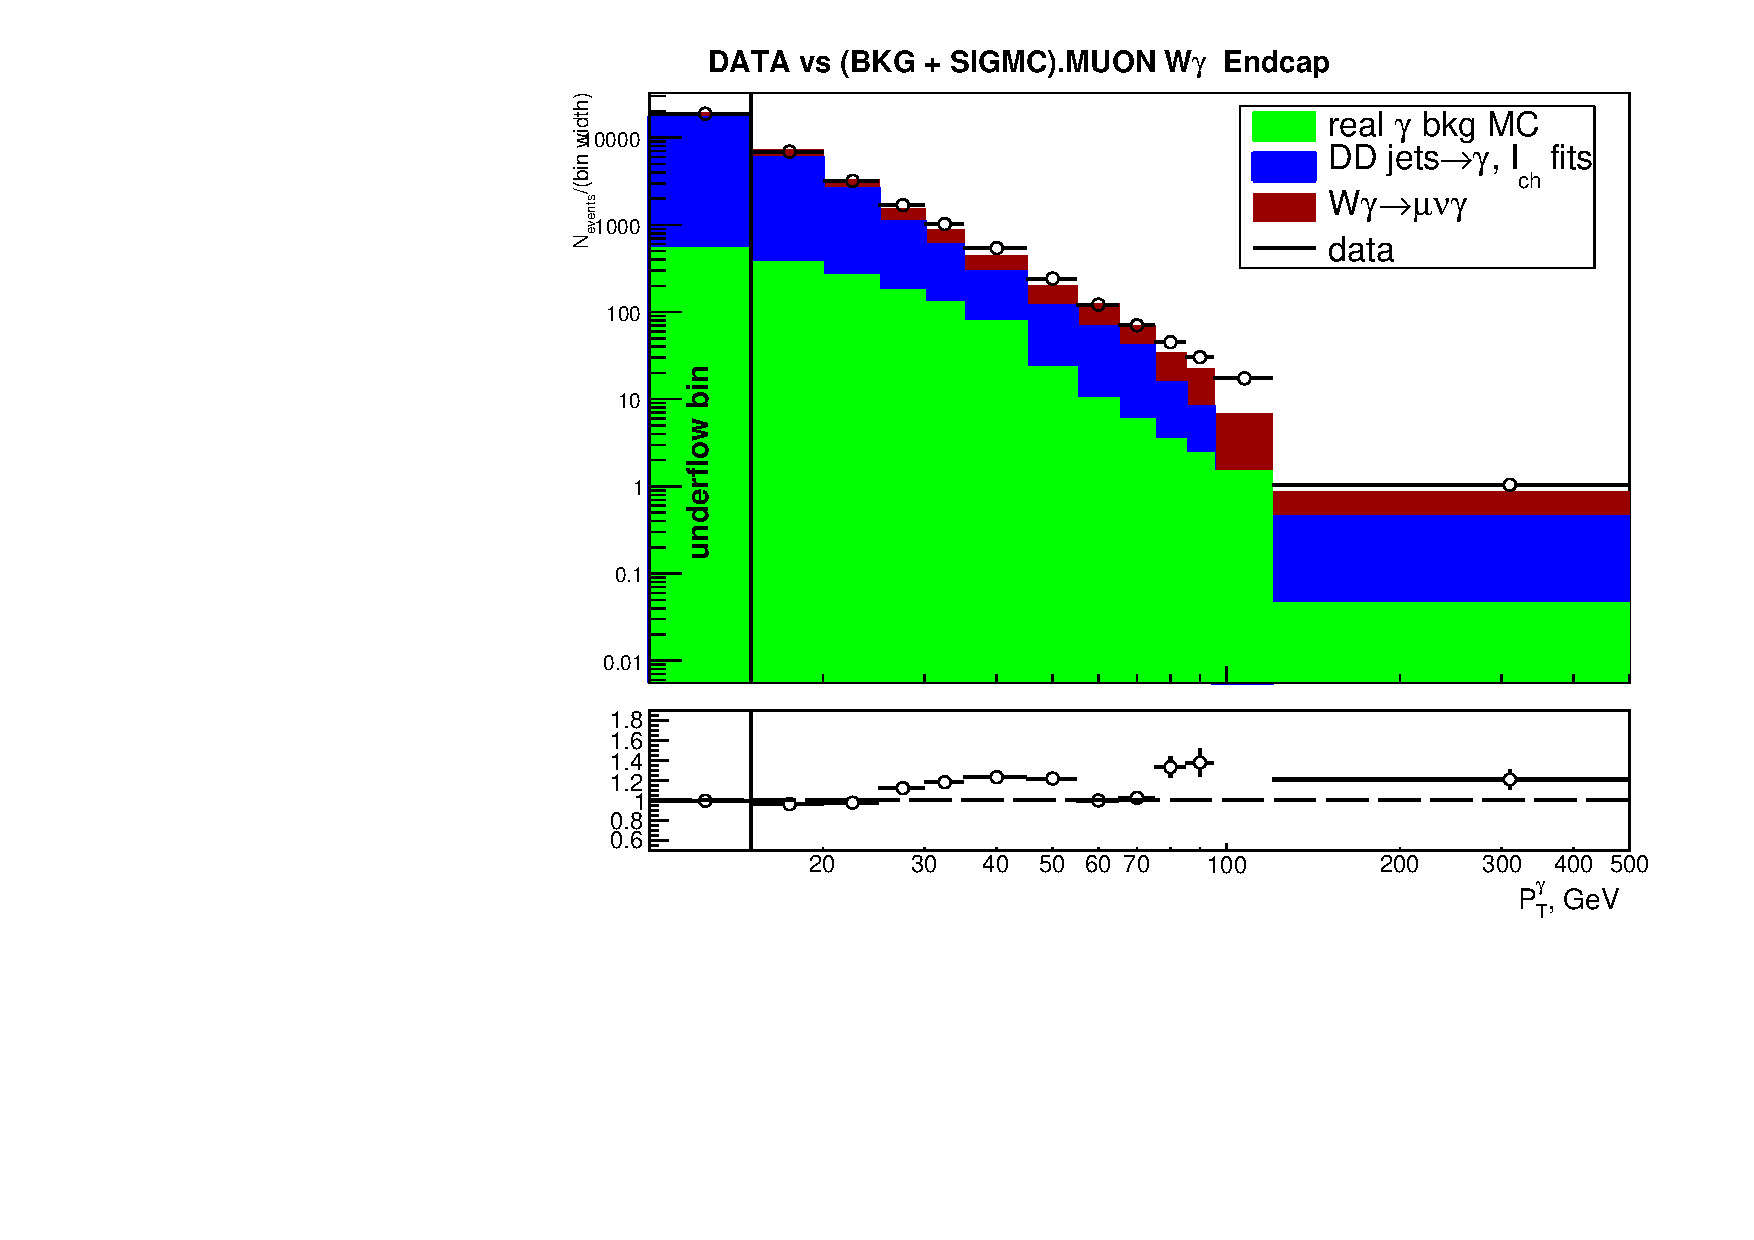
\includegraphics[width=0.45\textwidth]{../figs/figs_v11/MUON_WGamma/PrepareYields/c_DATAvsBkgPlusSigMCc_MUON_WGamma_TEMPL_CHISO_UNblind__Endcap__phoEt.pdf}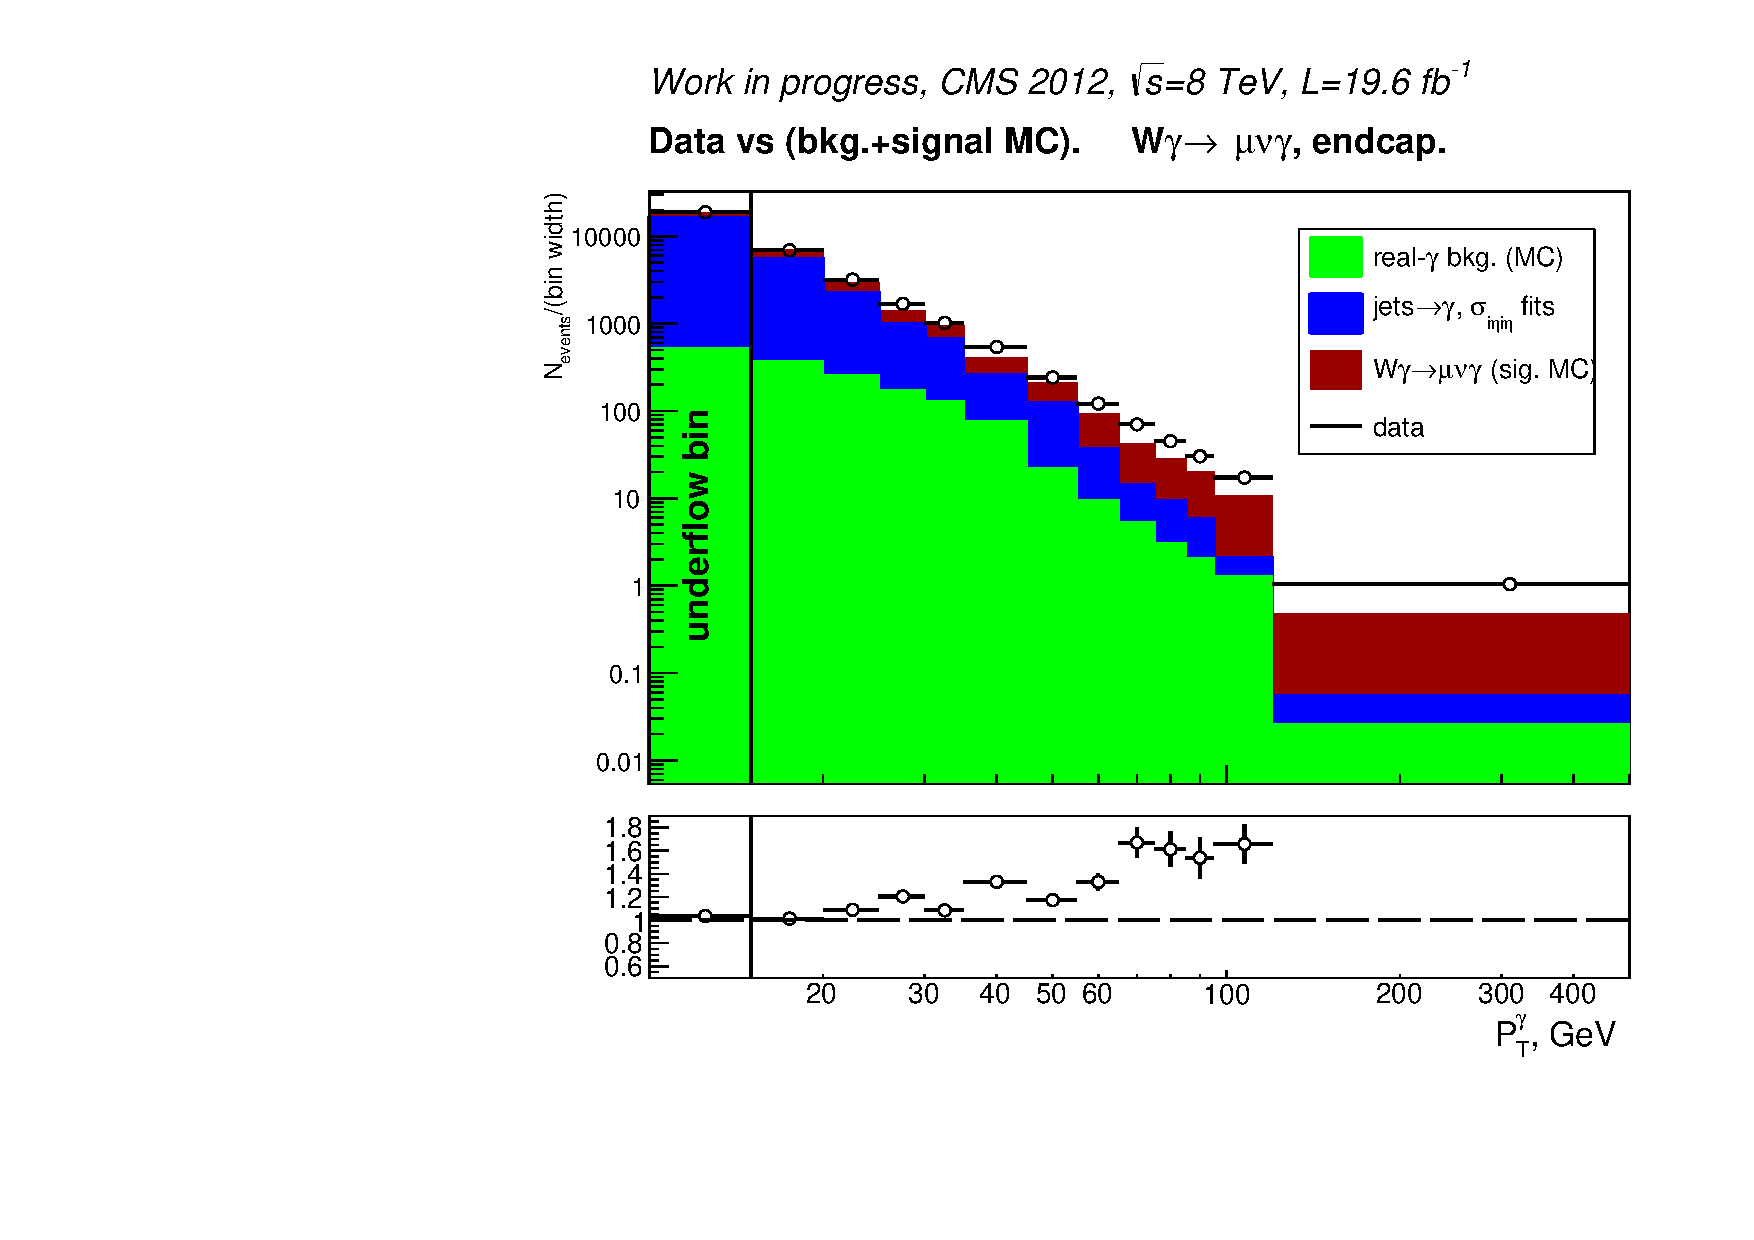
\includegraphics[width=0.45\textwidth]{../figs/figs_v11/MUON_WGamma/PrepareYields/c_DATAvsBkgPlusSigMCc_MUON_WGamma_TEMPL_SIHIH_UNblind__Endcap__phoEt.pdf}  \\
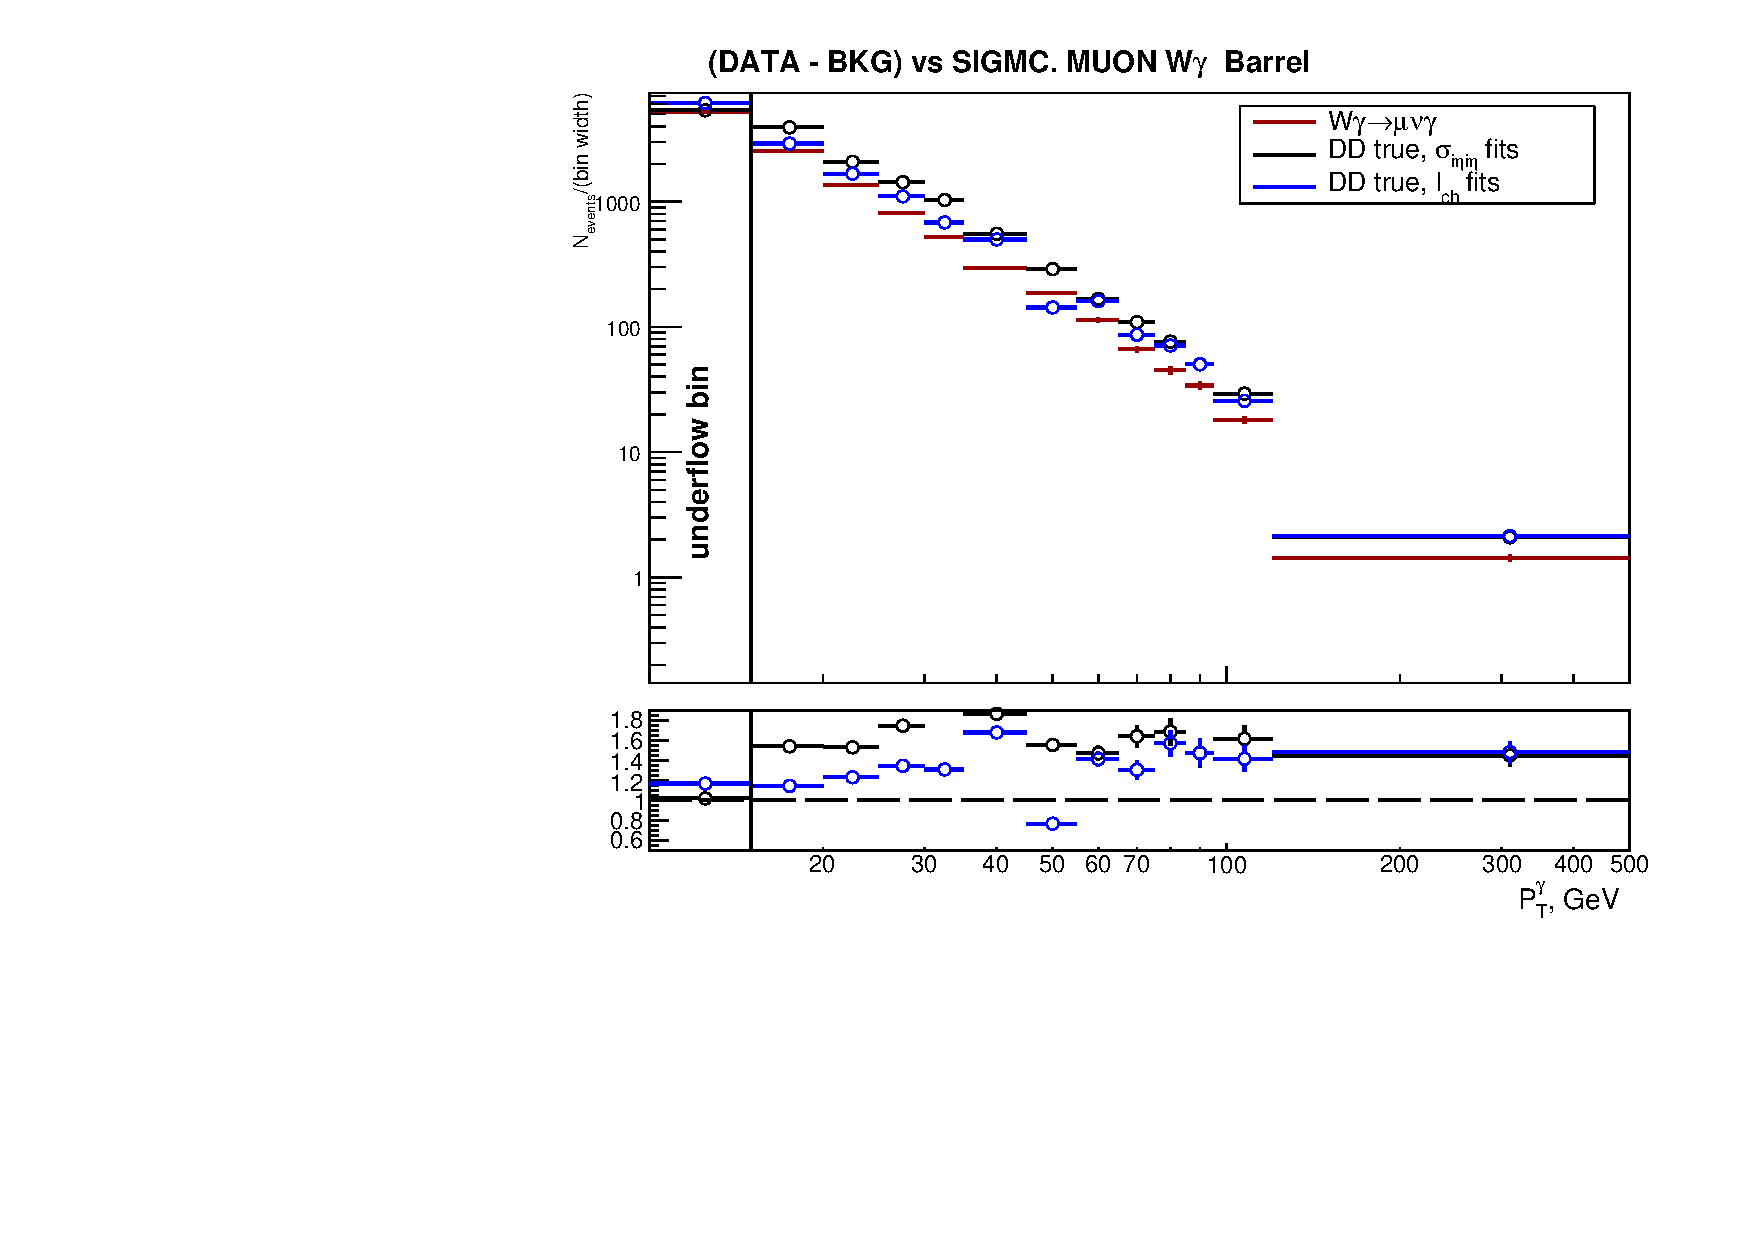
\includegraphics[width=0.45\textwidth]{../figs/figs_v11/MUON_WGamma/PrepareYields/c_BkgSubtrDATAvsSIGMC_c_MUON_WGamma__UNblind__Barrel__phoEt.pdf}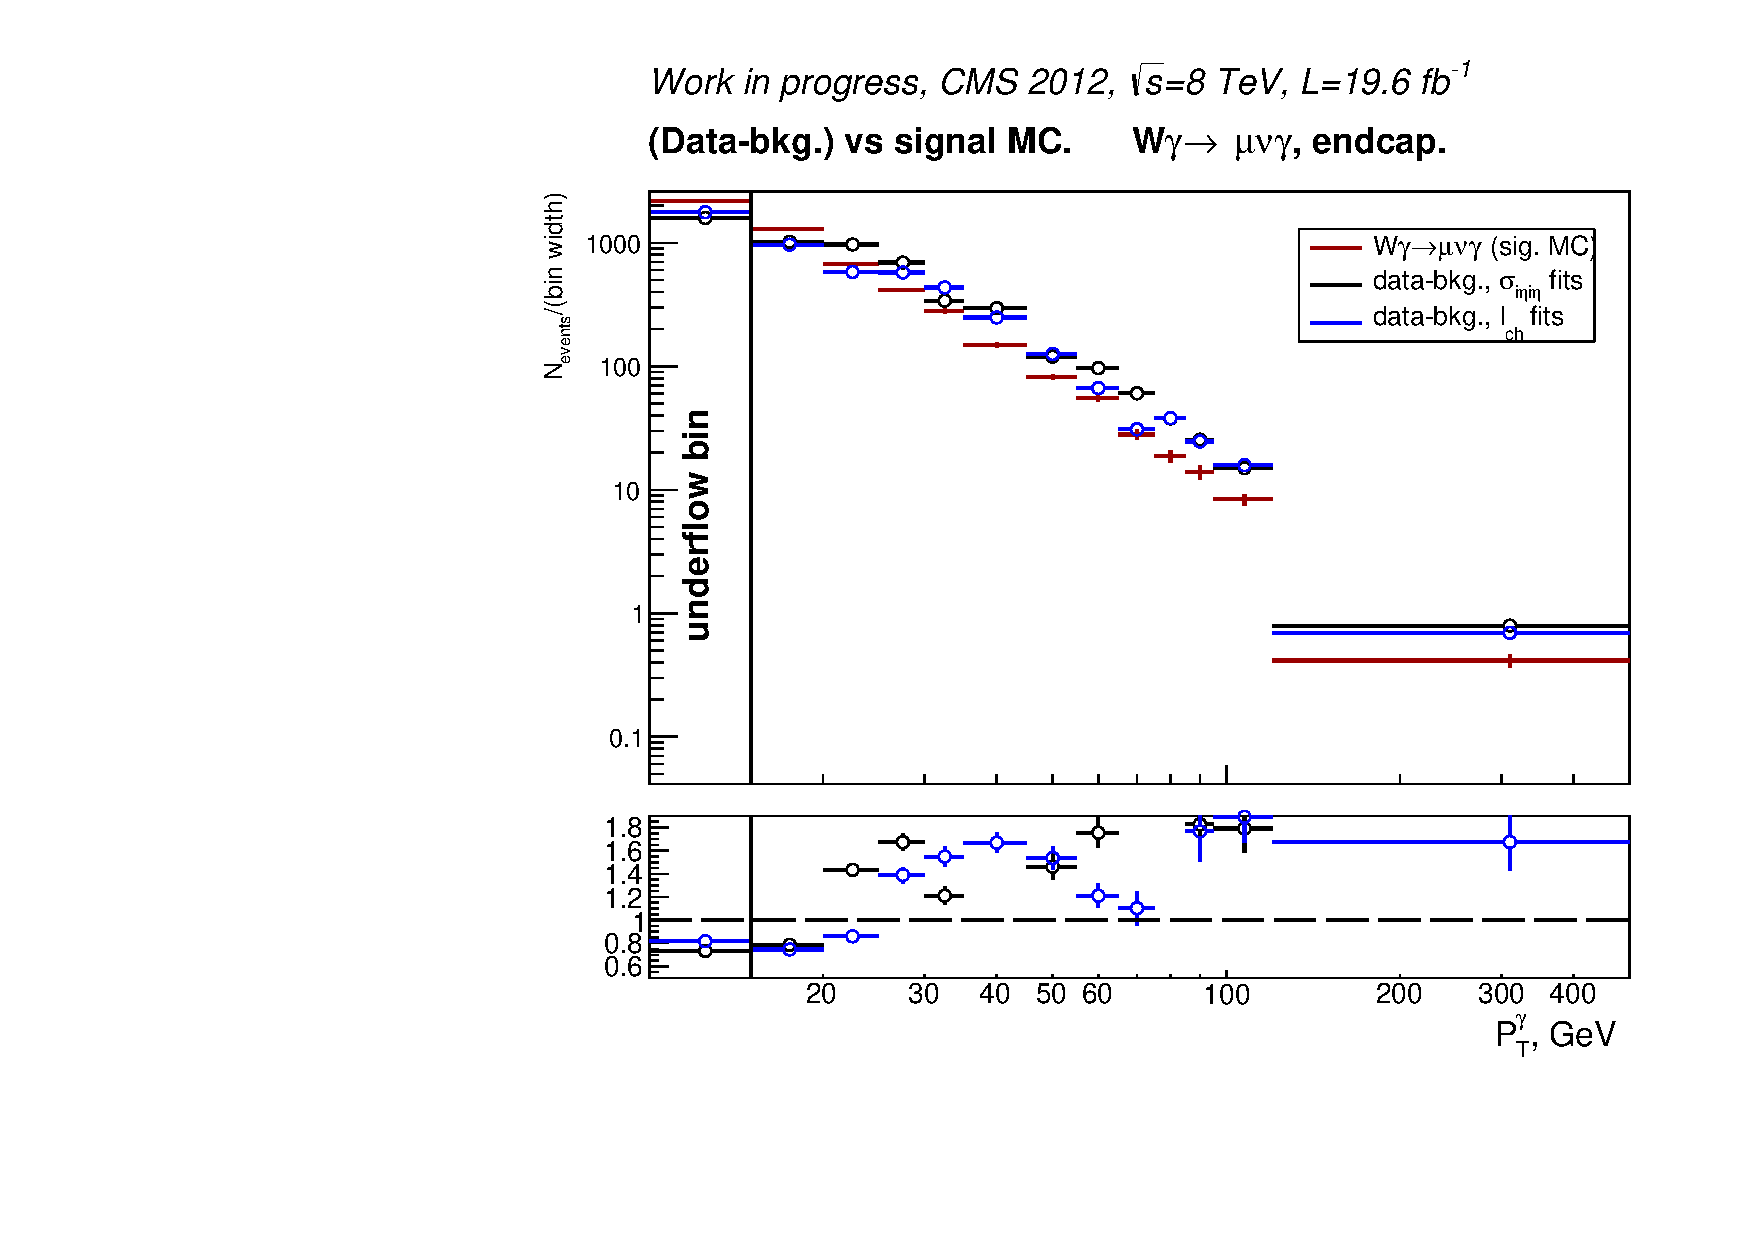
\includegraphics[width=0.45\textwidth]{../figs/figs_v11/MUON_WGamma/PrepareYields/c_BkgSubtrDATAvsSIGMC_c_MUON_WGamma__UNblind__Endcap__phoEt.pdf}\\
  \caption{Top and middle: data vs fake-$\gamma$ background derived from the template method + real-$\gamma$ background predicted by dedicated MC samples + signal MC, with $I_{ch}$ (left) and $\sigma_{i\eta i\eta}$ (right) used as fit variables in EB (top) and EE (middle). Bottom: data yields after full background subtraction vs signal MC in EB (left) and EE (right). $I_{ch}$ vs $\sigma_{i\eta i\eta}$ fit results. Muon channel.}
  \label{fig:DDvsMC_Wg_Data_MUON}
  \end{center}
\end{figure}

\begin{figure}[htb]
  \begin{center}
   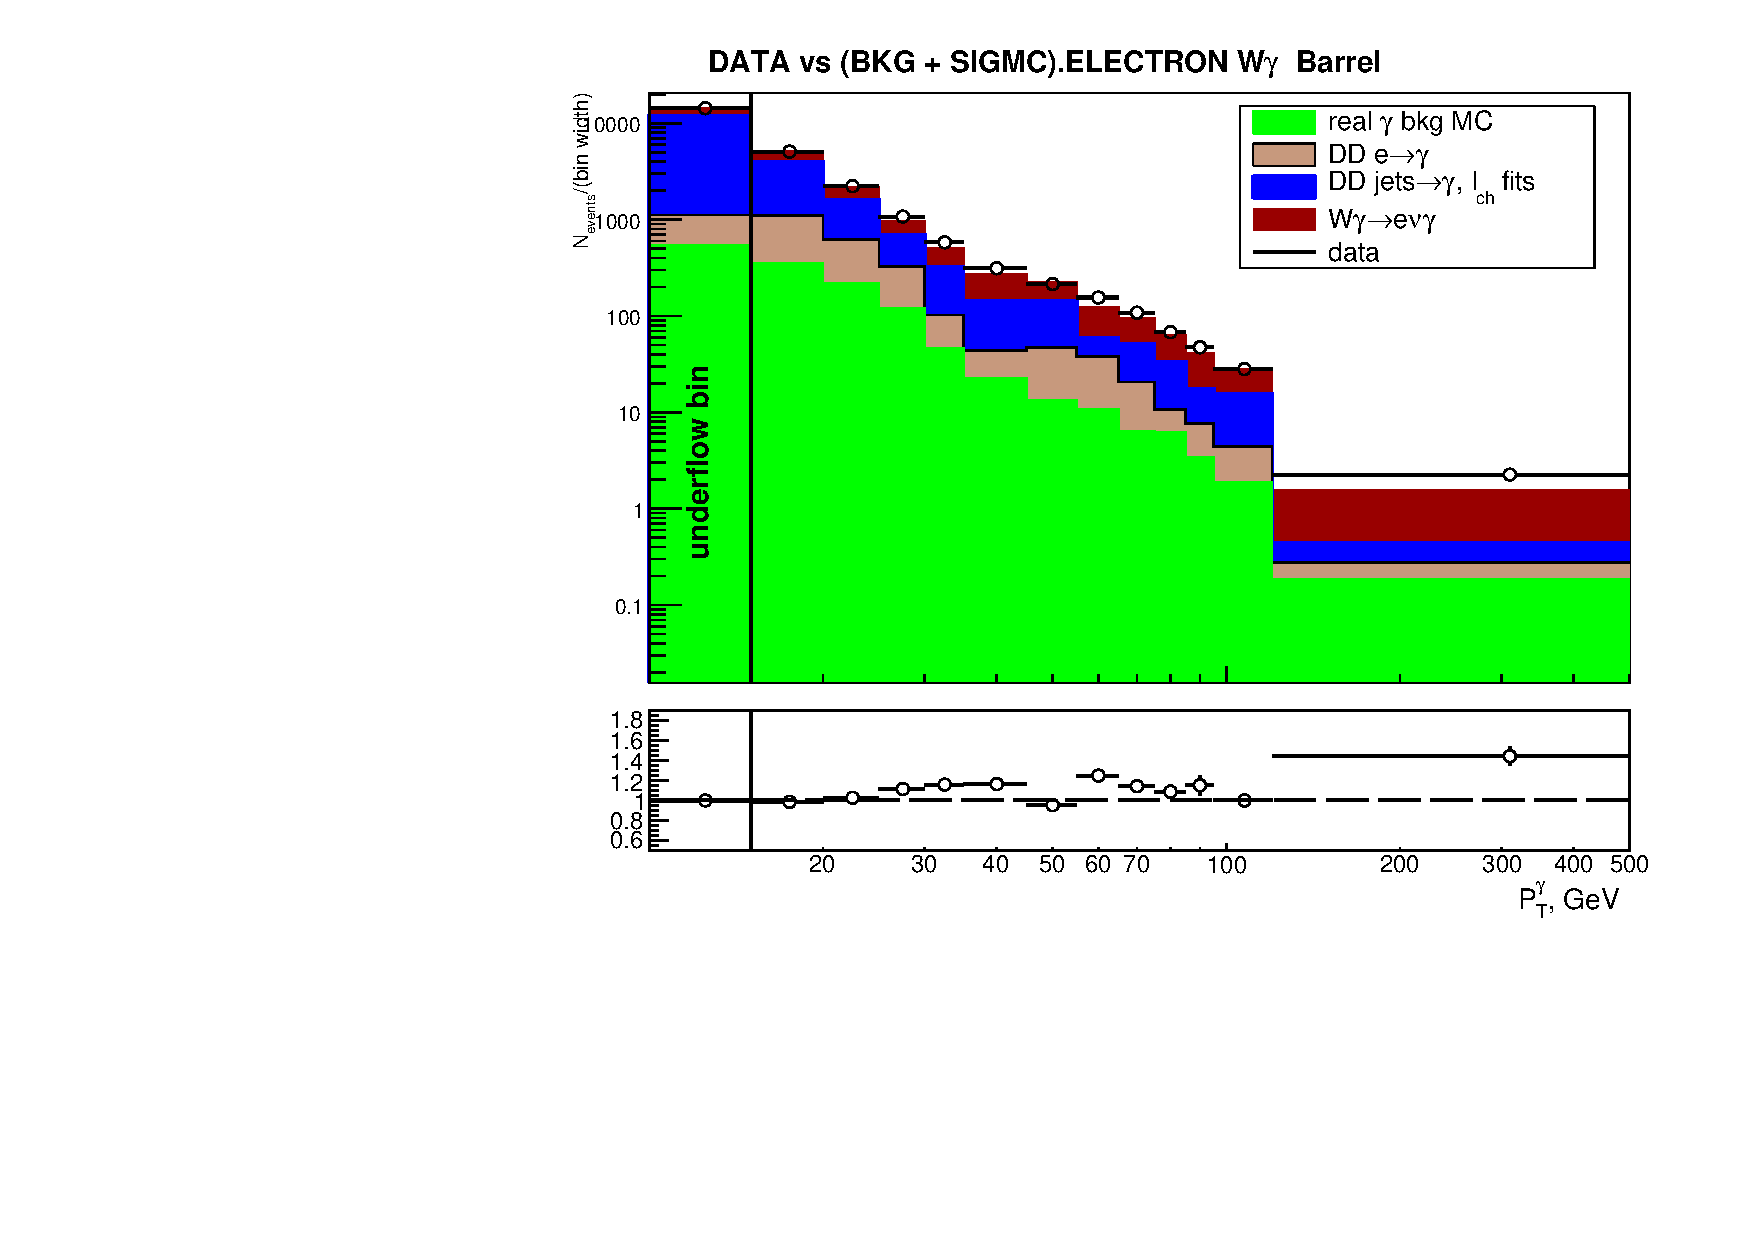
\includegraphics[width=0.45\textwidth]{../figs/figs_v11/ELECTRON_WGamma/PrepareYields/c_DATAvsBkgPlusSigMCc_ELECTRON_WGamma_TEMPL_CHISO_UNblind__Barrel__phoEt.pdf}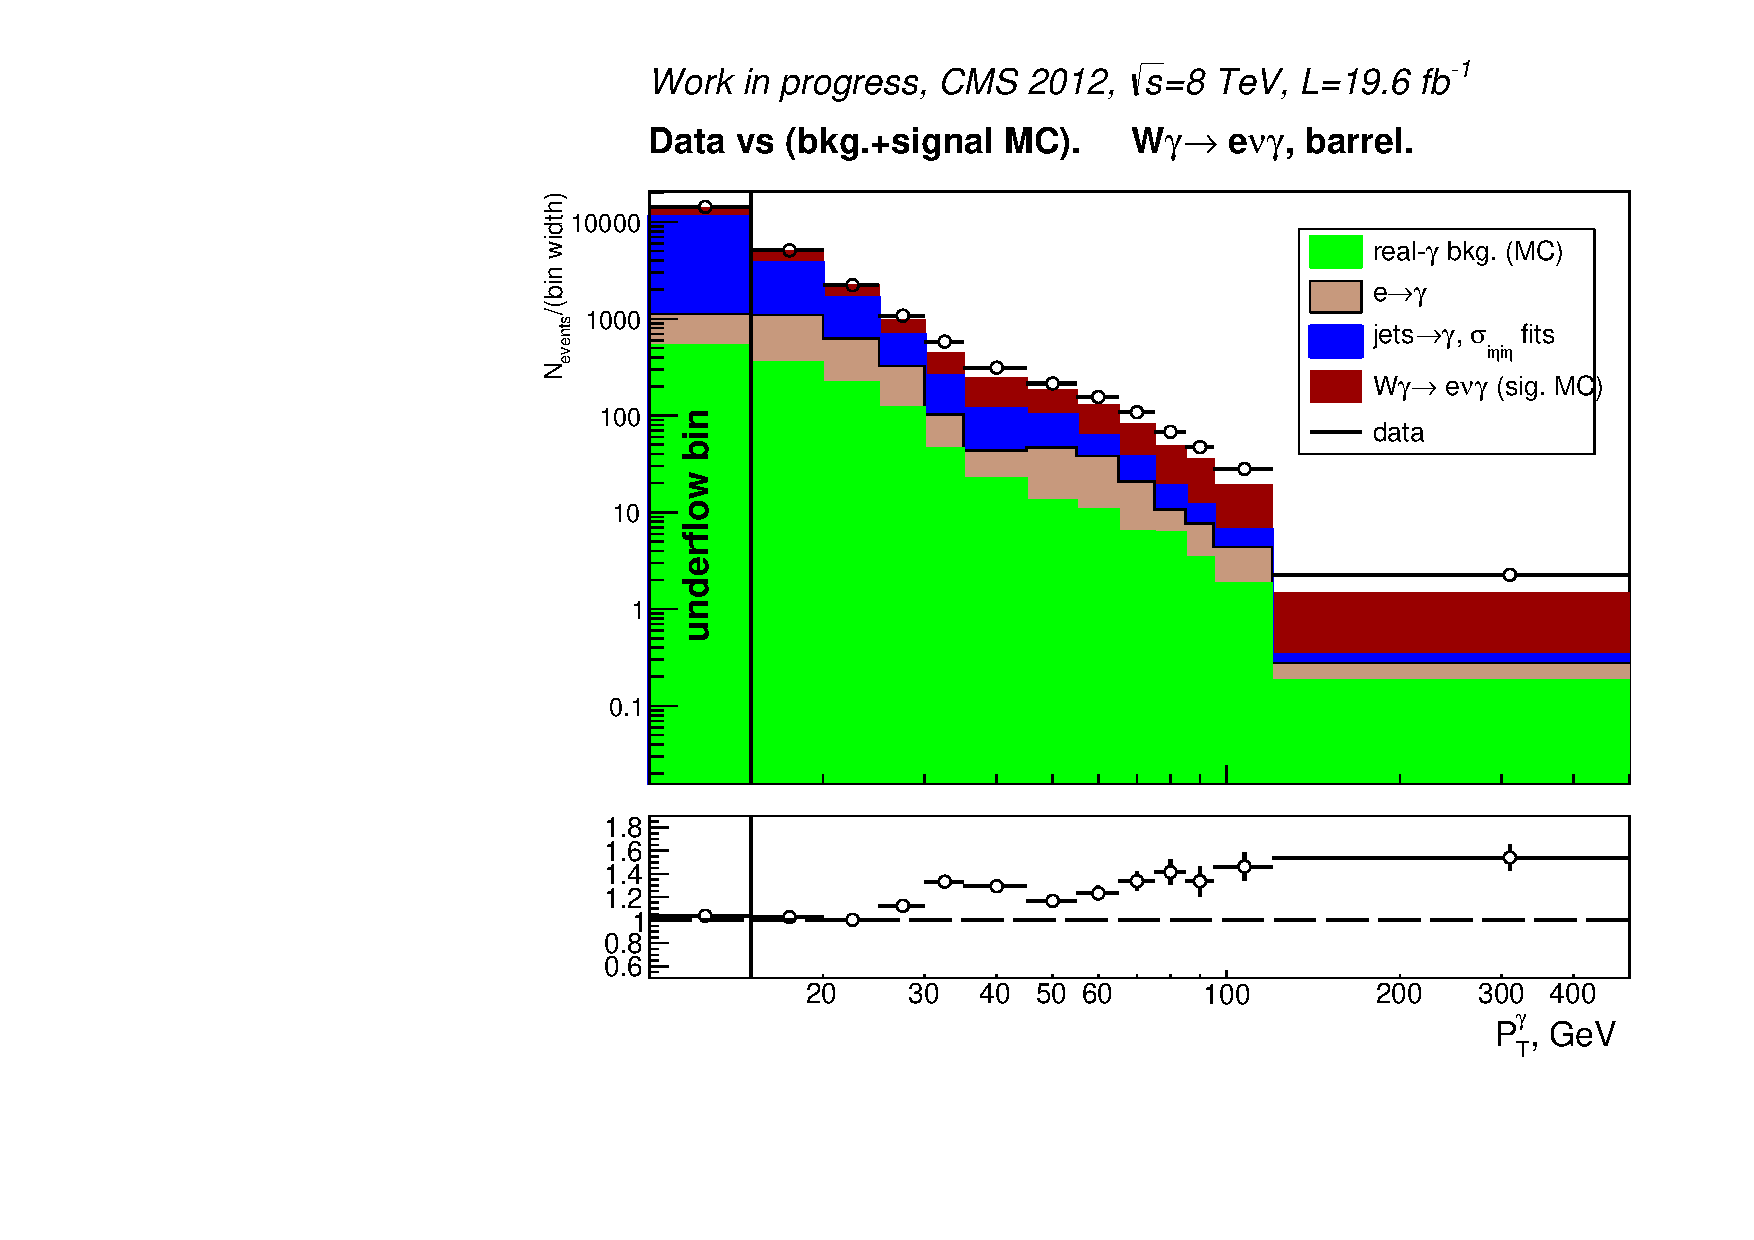
\includegraphics[width=0.45\textwidth]{../figs/figs_v11/ELECTRON_WGamma/PrepareYields/c_DATAvsBkgPlusSigMCc_ELECTRON_WGamma_TEMPL_SIHIH_UNblind__Barrel__phoEt.pdf}  \\
   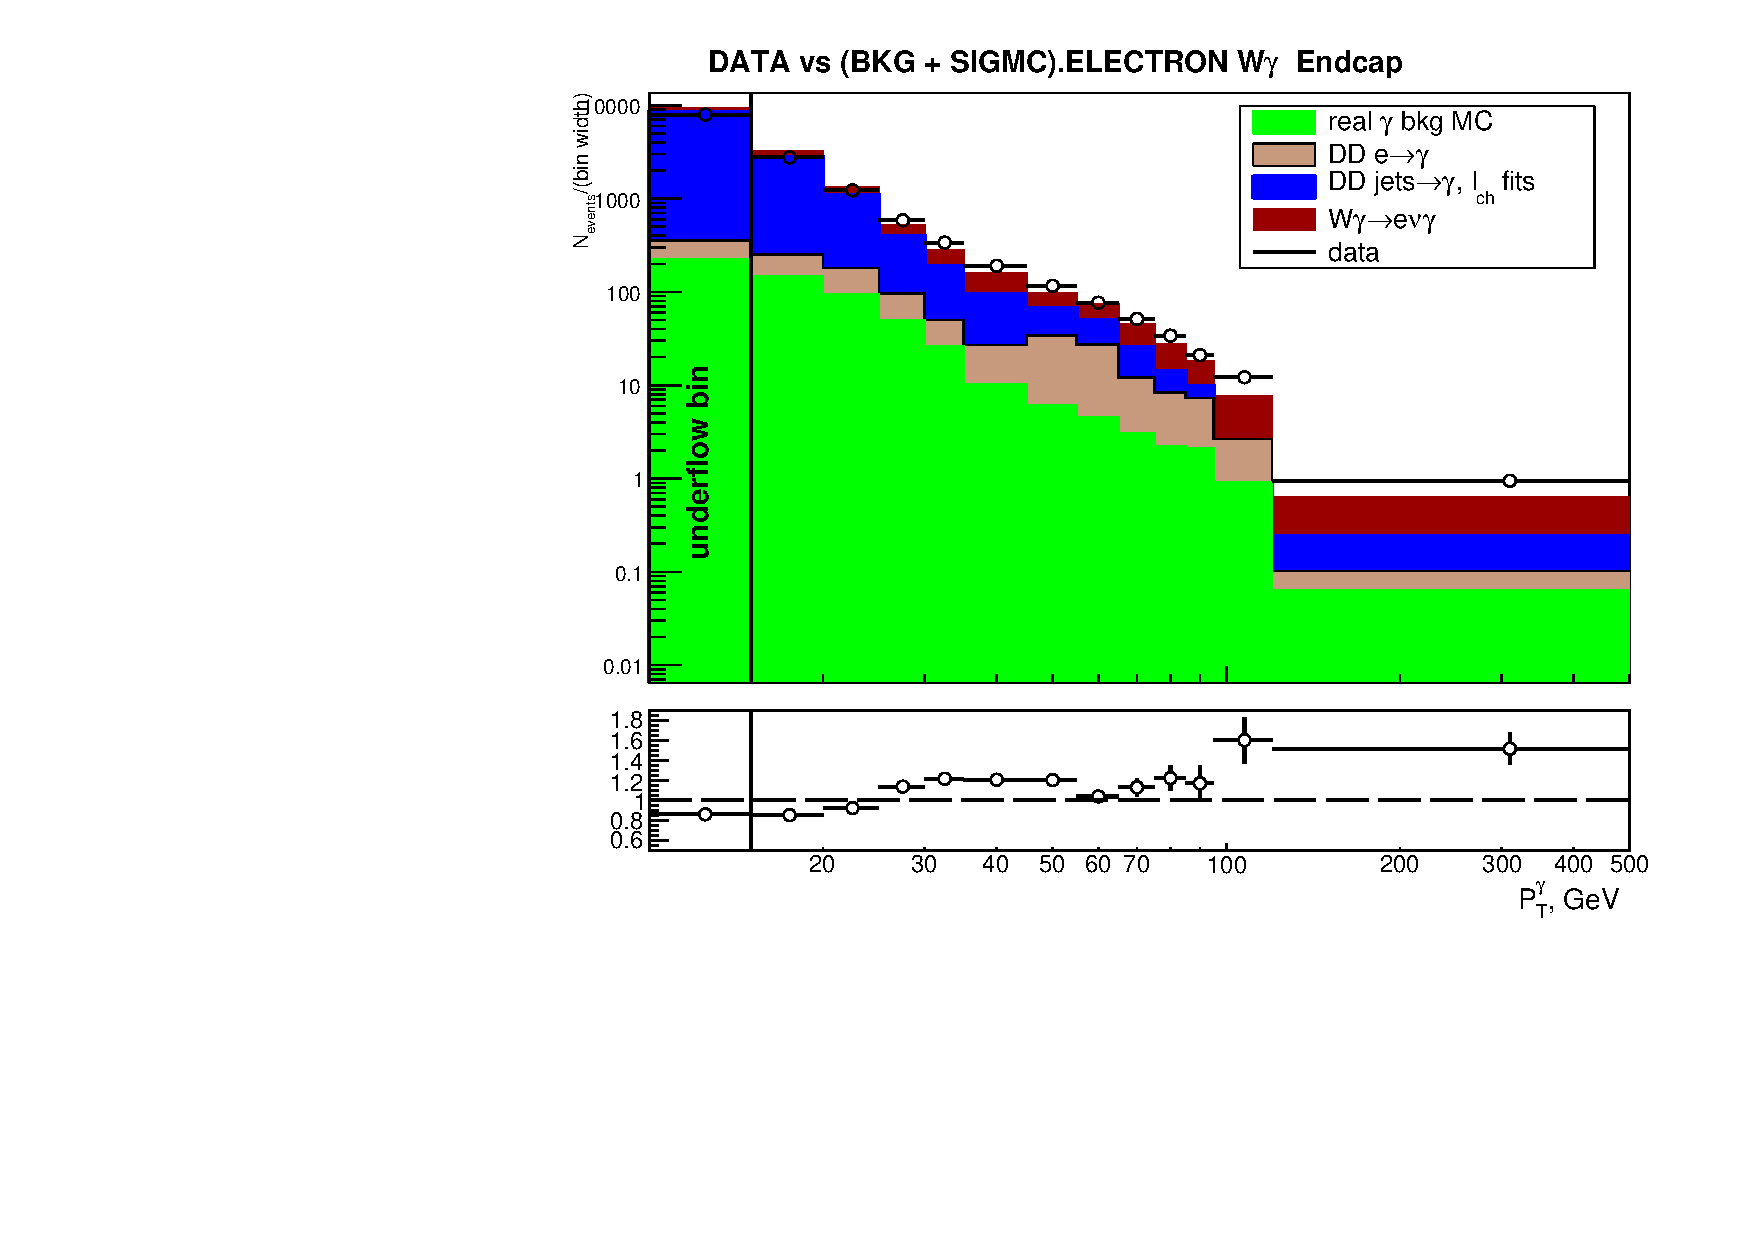
\includegraphics[width=0.45\textwidth]{../figs/figs_v11/ELECTRON_WGamma/PrepareYields/c_DATAvsBkgPlusSigMCc_ELECTRON_WGamma_TEMPL_CHISO_UNblind__Endcap__phoEt.pdf}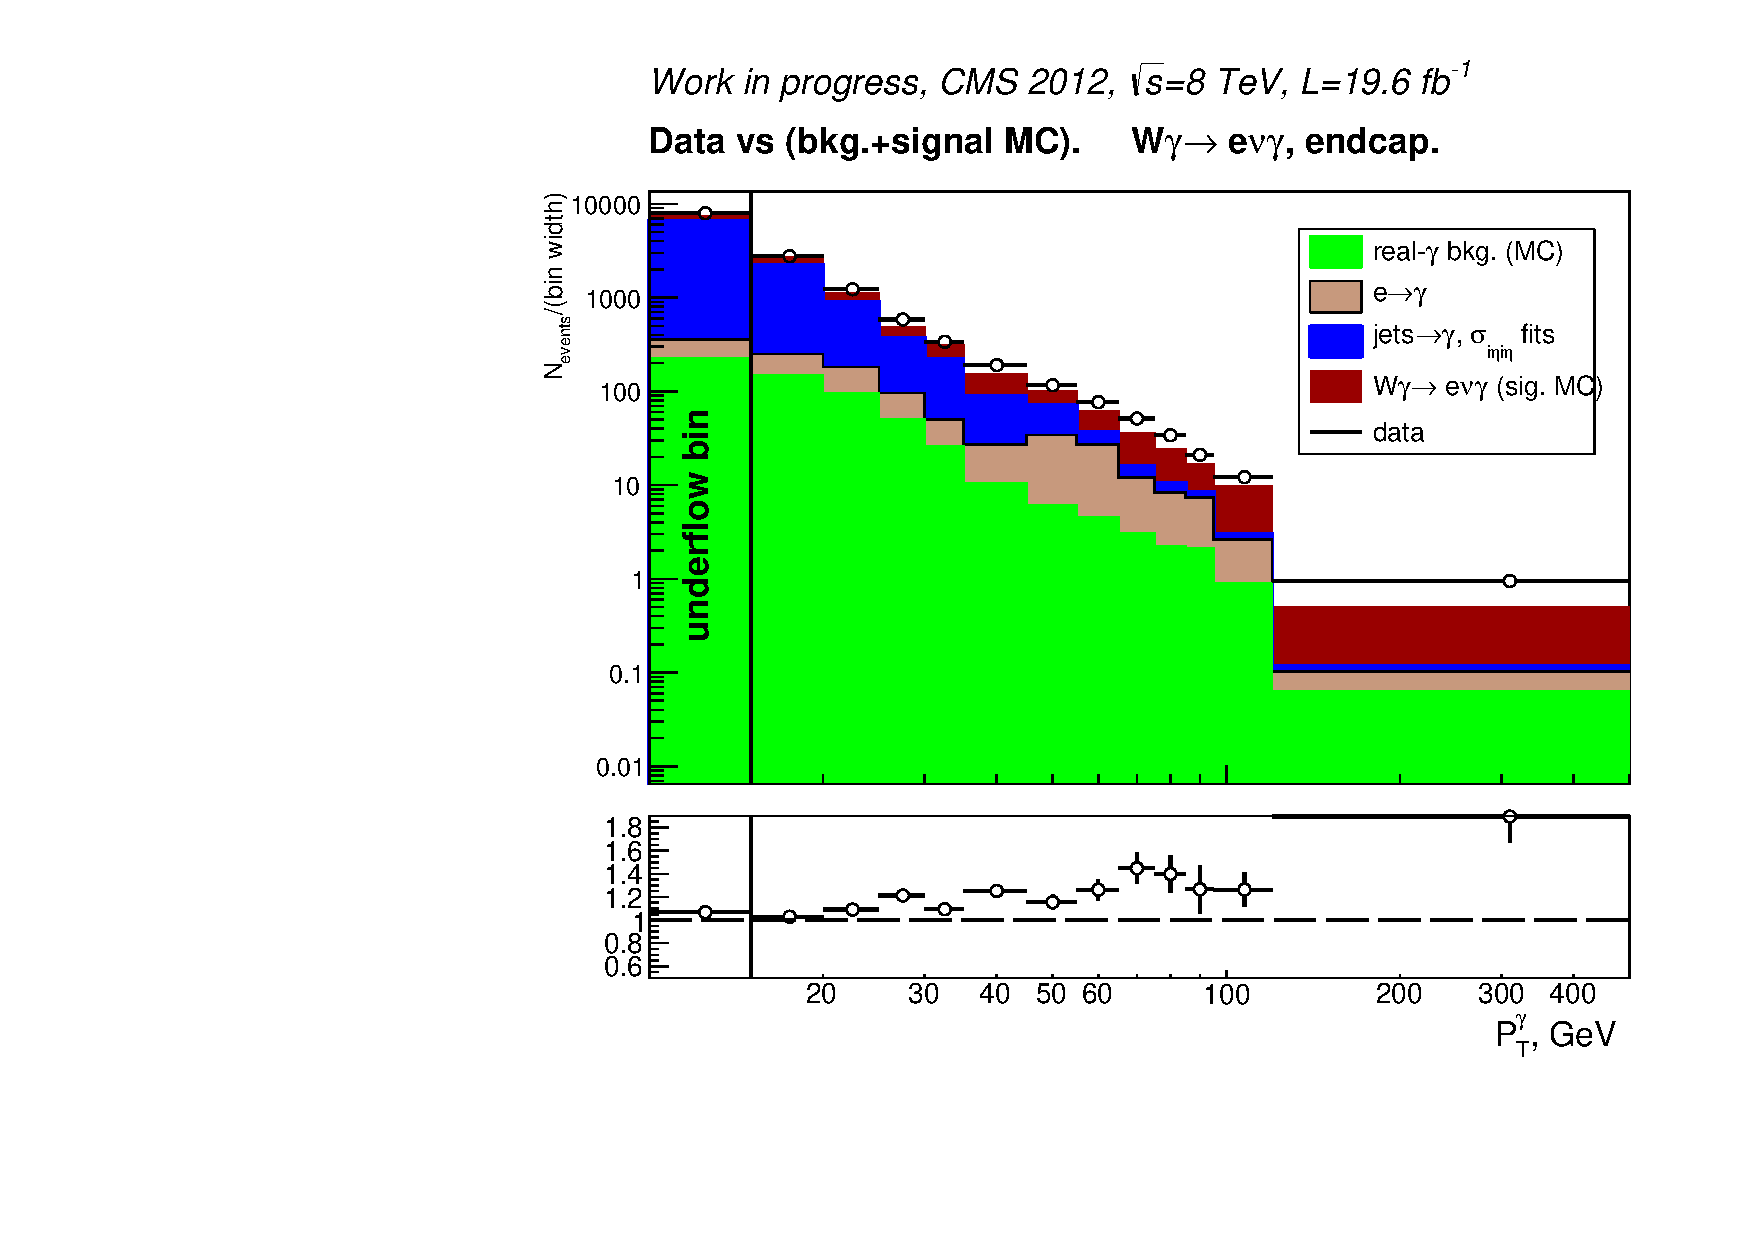
\includegraphics[width=0.45\textwidth]{../figs/figs_v11/ELECTRON_WGamma/PrepareYields/c_DATAvsBkgPlusSigMCc_ELECTRON_WGamma_TEMPL_SIHIH_UNblind__Endcap__phoEt.pdf}  \\
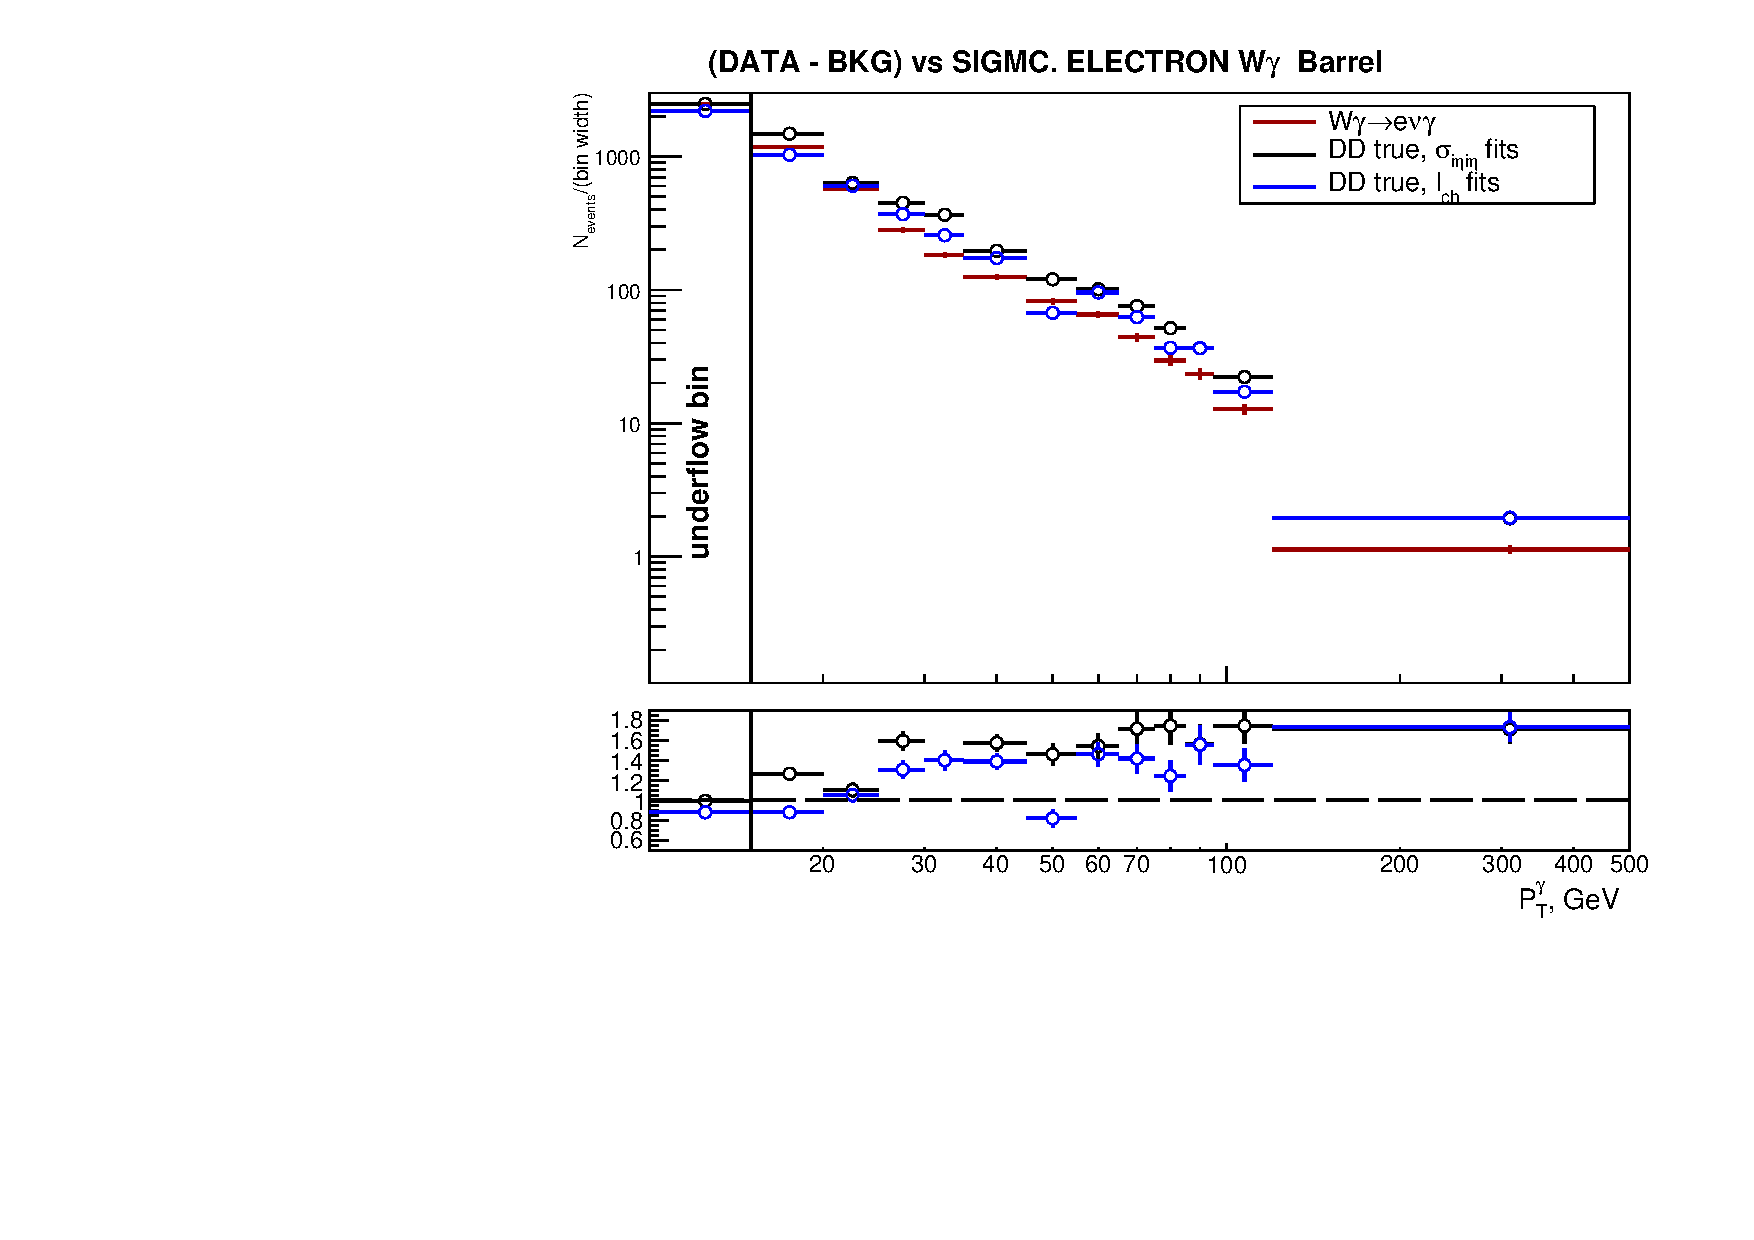
\includegraphics[width=0.45\textwidth]{../figs/figs_v11/ELECTRON_WGamma/PrepareYields/c_BkgSubtrDATAvsSIGMC_c_ELECTRON_WGamma__UNblind__Barrel__phoEt.pdf}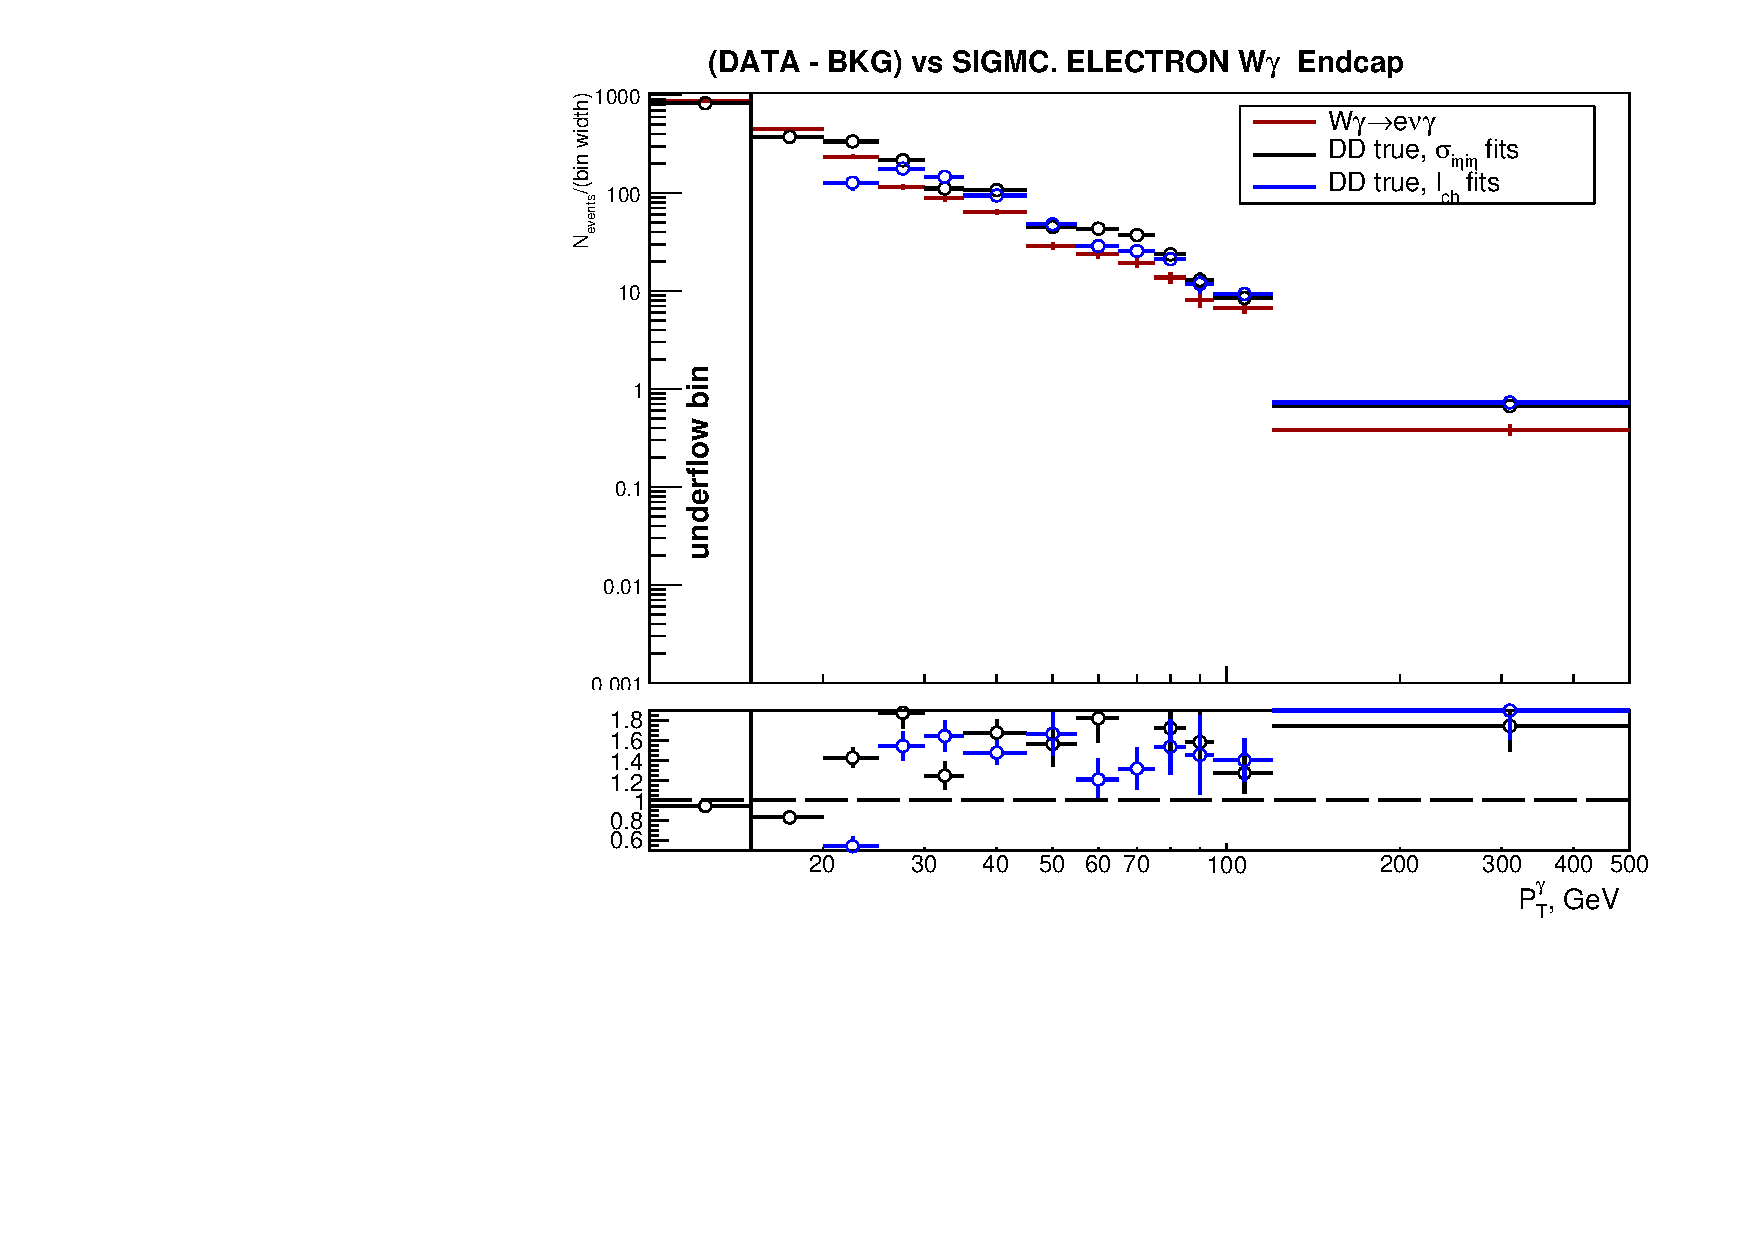
\includegraphics[width=0.45\textwidth]{../figs/figs_v11/ELECTRON_WGamma/PrepareYields/c_BkgSubtrDATAvsSIGMC_c_ELECTRON_WGamma__UNblind__Endcap__phoEt.pdf}\\
  \caption{Top and middle: data vs fake-$\gamma$ background derived from the template method + real-$\gamma$ background predicted by dedicated MC samples + signal MC, with $I_{ch}$ (left) and $\sigma_{i\eta i\eta}$ (right) used as fit variables in EB (top) and EE (middle). Bottom: data yields after full background subtraction vs signal MC in EB (left) and EE (right). $I_{ch}$ vs $\sigma_{i\eta i\eta}$ fit results. Electron channel.}
  \label{fig:DDvsMC_Wg_Data_ELECTRON}
  \end{center}
\end{figure}

\clearpage

\begin{table}[h]
  \scriptsize
  \begin{center}
  \caption{Data, signal and background yields. $W\gamma$, muon channel. First column is $P_T^{\gamma}$ ranges, second column is numbers of selected events in data in different $P_T^{\gamma}$ regions, third and fourth columns are estimates of the jets$\rightarrow\gamma$ background using $I_{ch}^{\gamma}$ and $\sigma_{i\eta i\eta}^{\gamma}$ templates, respectively, fifth column is MC-based estimates of the real-$\gamma$ background, sixth column is yields after the full background subtraction, and seventh column is signal MC predictions.}
  \begin{tabular}{|c|c|c|c|c|c|c|}
  \hline
                  &        &                 &                            &                   &           &   \\ 
    $P_T^{\gamma}$, & data   &  \multicolumn{3}{|c|}{background estimates}                      &  data-bkg & signal      \\ 
    GeV           & yields & \multicolumn{2}{|c|}{jets$\rightarrow\gamma$} & MC real-$\gamma$ &           & MC \\ 
                  &        & $I_{ch}^{\gamma$ & $\sigma_{i\eta i\eta}^{\gamma}$  &                  &           &   \\ \hline
\multicolumn{7}{|c|}{barrel photons}\\ \hline
10-15 & 114047$\pm$338 & 79833$\pm$251 & 77612$\pm$322 & 2453$\pm$46 & 26867$\pm$385 & 26251$\pm$240 \\ \hline 
15-20 & 41411$\pm$203 & 21434$\pm$150 & 24543$\pm$143 & 1566$\pm$34 & 19642$\pm$245 & 12707$\pm$164 \\ \hline 
20-25 & 19801$\pm$141 & 8466$\pm$101 & 9878$\pm$78 & 1283$\pm$31 & 10446$\pm$168 & 6793$\pm$120 \\ \hline 
25-30 & 11409$\pm$107 & 3509$\pm$68 & 4402$\pm$46 & 1180$\pm$27 & 7180$\pm$123 & 4087$\pm$93 \\ \hline 
30-35 & 7717$\pm$88 & 1687$\pm$49 & 2944$\pm$40 & 1253$\pm$27 & 5181$\pm$99 & 2604$\pm$75 \\ \hline 
35-45 & 9339$\pm$97 & 1947$\pm$56 & 2540$\pm$33 & 1840$\pm$33 & 5587$\pm$114 & 2971$\pm$80 \\ \hline 
45-55 & 3950$\pm$63 & 731$\pm$40 & 1964$\pm$40 & 477$\pm$18 & 2923$\pm$75 & 1861$\pm$63 \\ \hline 
55-65 & 2172$\pm$47 & 415$\pm$25 & 363$\pm$11 & 164$\pm$12 & 1694$\pm$50 & 1135$\pm$50 \\ \hline 
65-75 & 1320$\pm$36 & 177$\pm$17 & 466$\pm$19 & 81$\pm$8 & 1106$\pm$39 & 664$\pm$38 \\ \hline 
75-85 & 899$\pm$30 & 103$\pm$13 & 238$\pm$16 & 51$\pm$7 & 773$\pm$32 & 452$\pm$31 \\ \hline 
85-95 & 600$\pm$24 & 76$\pm$11 & 146$\pm$11 & 34$\pm$6 & 510$\pm$26 & 341$\pm$27 \\ \hline 
95-120 & 856$\pm$29 & 67$\pm$11 & 319$\pm$25 & 60$\pm$9 & 750$\pm$31 & 454$\pm$31 \\ \hline 
120-500 & 897$\pm$30 & 28$\pm$7 & 83$\pm$7 & 50$\pm$8 & 825$\pm$31 & 547$\pm$34 \\ \hline 
\multicolumn{7}{|c|}{endcap photons}\\ \hline
10-15 & 94370$\pm$307 & 77649$\pm$215 & 81161$\pm$426 & 2632$\pm$41 & 7937$\pm$306 & 10823$\pm$154 \\ \hline 
15-20 & 34643$\pm$186 & 25902$\pm$142 & 27661$\pm$184 & 1835$\pm$34 & 5089$\pm$213 & 6474$\pm$120 \\ \hline 
20-25 & 15988$\pm$126 & 10018$\pm$93 & 11659$\pm$102 & 1294$\pm$29 & 4842$\pm$138 & 3377$\pm$86 \\ \hline 
25-30 & 8429$\pm$92 & 4061$\pm$58 & 4558$\pm$51 & 871$\pm$23 & 3460$\pm$98 & 2068$\pm$67 \\ \hline 
30-35 & 5110$\pm$71 & 2669$\pm$54 & 2268$\pm$32 & 641$\pm$19 & 1700$\pm$81 & 1404$\pm$56 \\ \hline 
35-45 & 5414$\pm$74 & 1807$\pm$44 & 2113$\pm$29 & 771$\pm$22 & 2957$\pm$83 & 1489$\pm$57 \\ \hline 
45-55 & 2422$\pm$49 & 1025$\pm$50 & 936$\pm$19 & 222$\pm$13 & 1196$\pm$68 & 819$\pm$43 \\ \hline 
55-65 & 1217$\pm$35 & 270$\pm$19 & 564$\pm$16 & 94$\pm$9 & 966$\pm$36 & 551$\pm$35 \\ \hline 
65-75 & 703$\pm$27 & 87$\pm$11 & 346$\pm$13 & 54$\pm$7 & 604$\pm$28 & 280$\pm$25 \\ \hline 
75-85 & 451$\pm$21 & 63$\pm$9 & 117$\pm$6 & 30$\pm$5 & 379$\pm$22 & 186$\pm$20 \\ \hline 
85-95 & 303$\pm$17 & 37$\pm$7 & 56$\pm$4 & 21$\pm$5 & 255$\pm$18 & 139$\pm$18 \\ \hline 
95-120 & 433$\pm$21 & 20$\pm$5 & -81$\pm$5 & 32$\pm$6 & 374$\pm$21 & 209$\pm$22 \\ \hline 
120-500 & 396$\pm$20 & 11$\pm$4 & 153$\pm$12 & 10$\pm$2 & 302$\pm$18 & 157$\pm$19 \\ \hline 
  \end{tabular}
  \label{tab:yields_Wg_to_munu_}
  \end{center}
\end{table}

\clearpage

\begin{table}[h]
  \scriptsize
  \begin{center}
  \caption{Data, signal and background yields. $W\gamma$, electron channel. First column is $P_T^{\gamma}$ ranges, second column is numbers of selected events in data in different $P_T^{\gamma}$ regions, third and fourth columns are estimates of the jets$\rightarrow\gamma$ background using $I_{ch}^{\gamma}$ and $\sigma_{i\eta i\eta}^{\gamma}$ templates, respectively, fifth column is $e\rightarrow\gamma$ background estimates, sixths column is MC-based estimates of the real-$\gamma$ background, seventh column is yields after the full background subtraction, and eighth column is signal MC predictions.}
  \begin{tabular}{|c|c|c|c|c|c|c|c|}
                  &        &                 &                            & &                   &           &   \\ 
    $P_T^{\gamma}$, & data   &  \multicolumn{4}{|c|}{background estimates}                      &  data-bkg & signal      \\ 
    GeV           & yields & \multicolumn{2}{|c|}{jets$\rightarrow\gamma$} & $e\rightarrow\gamma$ & MC real-$\gamma$ &           & MC \\ 
                  &        & $I_{ch}^{\gamma$ & $\sigma_{i\eta i\eta}^{\gamma}$  &                       &                  &           &   \\ \hline
\multicolumn{8}{|c|}{barrel photons}\\ \hline
10-15 & 71649$\pm$268 & 51004$\pm$200 & 53577$\pm$266 & 2923$\pm$80 & 2688$\pm$41 & 12425$\pm$316 & 12480$\pm$164 \\ \hline
15-20 & 25455$\pm$160 & 13487$\pm$118 & 14474$\pm$110 & 3715$\pm$178 & 1779$\pm$32 & 7422$\pm$262 & 5858$\pm$110 \\ \hline
20-25 & 11130$\pm$105 & 5112$\pm$78 & 4846$\pm$55 & 2023$\pm$137 & 1101$\pm$25 & 3168$\pm$186 & 2869$\pm$77 \\ \hline
25-30 & 5388$\pm$73 & 1748$\pm$47 & 1790$\pm$29 & 1031$\pm$72 & 603$\pm$18 & 2251$\pm$111 & 1412$\pm$54 \\ \hline
30-35 & 2907$\pm$54 & 752$\pm$32 & 1079$\pm$24 & 286$\pm$33 & 229$\pm$12 & 1831$\pm$68 & 916$\pm$44 \\ \hline
35-45 & 3128$\pm$56 & 735$\pm$34 & 1003$\pm$21 & 215$\pm$27 & 223$\pm$12 & 1965$\pm$70 & 1248$\pm$51 \\ \hline
45-55 & 2147$\pm$46 & 551$\pm$31 & 964$\pm$28 & 335$\pm$37 & 134$\pm$10 & 1200$\pm$65 & 821$\pm$42 \\ \hline
55-65 & 1556$\pm$39 & 228$\pm$19 & 211$\pm$8 & 272$\pm$39 & 108$\pm$9 & 1011$\pm$57 & 654$\pm$37 \\ \hline
65-75 & 1083$\pm$33 & 163$\pm$16 & 300$\pm$15 & 143$\pm$27 & 64$\pm$7 & 757$\pm$44 & 441$\pm$31 \\ \hline
75-85 & 680$\pm$26 & 79$\pm$11 & 224$\pm$15 & 45$\pm$13 & 62$\pm$7 & 516$\pm$31 & 295$\pm$26 \\ \hline
85-95 & 473$\pm$22 & 43$\pm$9 & 99$\pm$9 & 43$\pm$17 & 34$\pm$5 & 366$\pm$29 & 234$\pm$23 \\ \hline
95-120 & 703$\pm$27 & 53$\pm$9 & 274$\pm$24 & 63$\pm$19 & 47$\pm$5 & 555$\pm$34 & 318$\pm$27 \\ \hline
120-500 & 859$\pm$29 & 23$\pm$6 & 61$\pm$6 & 34$\pm$12 & 71$\pm$8 & 735$\pm$33 & 430$\pm$31 \\ \hline
\multicolumn{8}{|c|}{endcap photons}\\ \hline
10-15 & 39746$\pm$199 & 31043$\pm$138 & 40022$\pm$13 & 666$\pm$38 & 1120$\pm$27 & 4130$\pm$204 & 4368$\pm$97 \\ \hline
15-20 & 13818$\pm$118 & 9920$\pm$88 & 12692$\pm$124 & 509$\pm$56 & 744$\pm$21 & 1870$\pm$145 & 2253$\pm$68 \\ \hline
20-25 & 6133$\pm$78 & 3538$\pm$56 & 4558$\pm$63 & 433$\pm$36 & 473$\pm$17 & 1680$\pm$92 & 1177$\pm$49 \\ \hline
25-30 & 2924$\pm$54 & 1358$\pm$34 & 1516$\pm$29 & 229$\pm$24 & 250$\pm$12 & 1079$\pm$62 & 575$\pm$34 \\ \hline
30-35 & 1690$\pm$41 & 850$\pm$31 & 694$\pm$18 & 120$\pm$16 & 130$\pm$9 & 555$\pm$49 & 445$\pm$31 \\ \hline
35-45 & 1905$\pm$44 & 613$\pm$26 & 670$\pm$16 & 167$\pm$19 & 103$\pm$8 & 1071$\pm$51 & 638$\pm$37 \\ \hline
45-55 & 1162$\pm$34 & 377$\pm$30 & 337$\pm$11 & 281$\pm$28 & 61$\pm$6 & 450$\pm$53 & 287$\pm$24 \\ \hline
55-65 & 767$\pm$28 & 98$\pm$12 & 228$\pm$11 & 227$\pm$28 & 46$\pm$6 & 433$\pm$40 & 238$\pm$22 \\ \hline
65-75 & 513$\pm$23 & 40$\pm$8 & 139$\pm$9 & 90$\pm$18 & 31$\pm$4 & 372$\pm$29 & 194$\pm$21 \\ \hline
75-85 & 340$\pm$18 & 22$\pm$6 & 57$\pm$5 & 62$\pm$15 & 22$\pm$5 & 236$\pm$24 & 137$\pm$18 \\ \hline
85-95 & 210$\pm$14 & 11$\pm$4 & 25$\pm$3 & 52$\pm$19 & 21$\pm$3 & 129$\pm$24 & 81$\pm$14 \\ \hline
95-120 & 304$\pm$17 & 8$\pm$3 & -43$\pm$4 & 43$\pm$13 & 23$\pm$5 & 212$\pm$22 & 166$\pm$20 \\ \hline
120-500 & 360$\pm$19 & 5$\pm$3 & 53$\pm$7 & 15$\pm$7 & 24$\pm$4 & 254$\pm$18 & 146$\pm$19 \\ \hline
  \end{tabular}
  \label{tab:yields_Wg_to_enu_}
  \end{center}
\end{table}
